\documentclass[11pt,a4paper]{article}

% ---------------------------------------------------------------------------
% Packages
% ---------------------------------------------------------------------------
\usepackage[T1]{fontenc}
\usepackage{lmodern}
\usepackage{amsmath,amssymb,amsthm,mathtools}
\usepackage{booktabs,tabularx,multirow,array}
\usepackage{xcolor}
\usepackage{microtype}
\usepackage[shortlabels]{enumitem}
\usepackage[margin=1in]{geometry}
\usepackage{tikz}
\usepackage{pgfplots}
\pgfplotsset{compat=1.18}
\usetikzlibrary{arrows.meta,positioning,shapes.geometric,fit,calc,decorations.pathreplacing}
\usepackage[font=small,labelfont=bf]{caption}
\usepackage[colorlinks=true,linkcolor=blue!50!black,citecolor=green!35!black,urlcolor=blue!50!black,hypertexnames=false]{hyperref}
\usepackage[capitalise,nameinlink]{cleveref}

% ---------------------------------------------------------------------------
% Theorem environments
% ---------------------------------------------------------------------------
\theoremstyle{plain}
\newtheorem{theorem}{Theorem}[section]
\newtheorem{proposition}[theorem]{Proposition}
\newtheorem{lemma}[theorem]{Lemma}
\newtheorem{corollary}[theorem]{Corollary}
\newtheorem{conjecture}[theorem]{Conjecture}
\theoremstyle{definition}
\newtheorem{definition}[theorem]{Definition}
\newtheorem{example}[theorem]{Example}
\theoremstyle{remark}
\newtheorem{remark}[theorem]{Remark}

% ---------------------------------------------------------------------------
% Notation
% ---------------------------------------------------------------------------
\newcommand{\Z}{\mathbb{Z}}
\newcommand{\Q}{\mathbb{Q}}
\newcommand{\R}{\mathbb{R}}
\newcommand{\C}{\mathbb{C}}
\newcommand{\F}{\mathbb{F}}
\newcommand{\PP}{\mathbb{P}}
\newcommand{\Oc}{\mathcal{O}}
\newcommand{\ind}{\operatorname{ind}}
\newcommand{\rk}{\operatorname{rk}}
\newcommand{\spn}{\operatorname{span}}
\newcommand{\conv}{\operatorname{conv}}
\newcommand{\Sym}{\operatorname{Sym}}
\newcommand{\tr}{\operatorname{tr}}
\newcommand{\Gam}{\Gamma}
\newcommand{\st}[1]{\textsf{\small #1}}          % logical status / verdict labels
\newcommand{\bfive}{\overline{\mathbf{5}}}
\newcommand{\ten}{\mathbf{10}}
\newcommand{\five}{\mathbf{5}}
\newcommand{\Xa}{X_{7862}}
\newcommand{\Xb}{X_{7447}}

\title{\textbf{Certified branch-and-bound for heterotic line-bundle standard models}\\[4pt]
\large Complete slope obstructions, charge-unbounded slices, first-principles
equivariant descent, and the holomorphic Yukawa sector}

\author{[Author names and affiliations]}
\date{\today}

\begin{document}
\maketitle

\begin{abstract}
We treat the construction of $E_8\times E_8$ heterotic compactifications on
favourable complete-intersection Calabi--Yau threefolds, with gauge bundle a sum
of five line bundles, as an exact search over integer charge matrices in which
every pruning decision is a proof and every outcome carries its logical status.
The central tool is a complete, coefficient-unbounded form of the slope
(poly-stability) obstruction: it holds exactly when the span of the charge
vectors meets a fixed polyhedral cone, it is monotone and so prunes every branch
of the search tree, and it is decided by a Gordan-type dual test whose cost falls
with depth; it removes a spurious candidate retained by the finite test of
earlier scans. A slice decomposition with a per-slice anomaly bound turns an
explicit family of slices into searches \emph{with no charge cutoff}---425 of
469 slices of the tetraquadric are proven empty for arbitrarily large
charges---and an index-divisibility obstruction gives the only fully unbounded
exclusions, both confirmed by the published catalog. The engine reproduces the
published GUT catalogs of the tetraquadric (10 and 58 models) and of CICY 7447
(93 models) exactly, independent replays exhaust domains of up to
$3.5\times10^9$ states, and run over all 68 favourable CICYs it
recovers every published model inside its search boxes. An exact Gröbner and
interval-arithmetic decision of stability, itself checked never to reject a
published model, classifies the extra survivors and certifies one poly-stable
GUT model that the published catalog misses. Computing the $\Gam$-representation on cohomology from
the group action (reproducing all 27,821 published character tables exactly), we
search rather than verify: 21 orbits on the
tetraquadric quotient admit three chiral families, no charged exotics and a Higgs
pair, 11 of them absent from the published standard-model database---each
because it lies outside that scan's own stated domain. Treating the $U(1)^4$
selection rules exactly, as network-flow membership, we reproduce every operator
table of that database for all 2,012 models and find 954 of 2,007 down-type
Yukawa tables internally inconsistent. Evaluating leading-order couplings as
cohomological triple products, independent of complex structure, and running new
and published models through one pipeline, we find that no model on the quotient
combines a leading-order top Yukawa, rank-three Yukawa matrices and the absence
of dangerous operators; the new models fail for the same reasons, at a similar
rate, as the published ones.
\end{abstract}

\setcounter{tocdepth}{1}
\tableofcontents
\bigskip

\section{Introduction}
\label{sec:intro}

Heterotic compactifications on smooth Calabi--Yau threefolds with gauge bundles
built from sums of line bundles are among the most successful constructions of
string vacua with the charged spectrum of the minimal supersymmetric Standard
Model (MSSM)~\cite{AGLP2011,AGLP2012,ACGLP2013}. The construction is
combinatorial at its core. On a favourable complete-intersection Calabi--Yau
(CICY) threefold $X$ with $h\coloneqq h^{1,1}(X)$, a rank-five bundle
$V=\bigoplus_{a=1}^{5}\Oc_X(k_a)$ is determined by an integer $h\times 5$ charge
matrix $K=(k_1,\dots,k_5)$, and the conditions for a consistent, supersymmetric
$SU(5)$ grand unified theory with three chiral families---vanishing first Chern
class, the correct chiral index, the Green--Schwarz anomaly condition and
poly-stability---are conditions on $K$ and on the topological data of $X$.
Descending to a Standard-Model-like theory then requires a freely acting
symmetry $\Gam$, an equivariant structure on $V$ and a Wilson line.

Earlier work turned this into a systematic scan: \cite{ACGLP2013} enumerated all
bundles on the 68 favourable CICYs with $h\le 6$ whose charges lie in a finite
box, producing a catalog of 63,325 GUT models, and \cite{AGLP2011,AGLP2012}
produced a database of downstairs standard models together with their
superpotential selection rules. Machine-learning and heuristic optimisers have
since been applied to the same space~\cite{ACHLN2023}. These are powerful, but
they leave three questions open that this paper addresses.

\paragraph{What does a negative search result prove?} A scan over a charge box
$|k_a^i|\le K$ that finds nothing establishes, at best, a statement about that
box, and only if every filter used to discard candidates is a genuine
\emph{necessary} condition. Several filters in the literature are finite
truncations of conditions that quantify over infinite sets (the slope
obstruction quantifies over all integer combinations of the charge vectors), and
whether their truncations are sound, complete or neither has not, to our
knowledge, been settled. Nor is it obvious which parts of the landscape can be
excluded \emph{without} a charge cutoff.

\paragraph{Can the downstairs spectrum be computed, not looked up?} The
$\Gam$-representation content of bundle cohomology decides which states survive
the quotient. In existing databases it is supplied as data. A search that
discovers new downstairs models needs to compute it from the group action.

\paragraph{What does the superpotential actually do?} Charge conservation under
the $U(1)^4$ remnant of the structure group is a necessary condition for a
coupling. It is not sufficient: a coupling allowed by the charges can vanish
for cohomological reasons. Distinguishing the two needs the actual cup product.

\subsection{Summary of results}

We build a search engine whose outputs carry their precise logical status and
whose every pruning decision is a proof, and use it to answer these questions
on the two benchmark geometries of~\cite{ACGLP2013}, the tetraquadric
$\Xa$ ($h=4$) and $\Xb$ ($h=5$). The main results are:

\begin{enumerate}[leftmargin=*,label=\textbf{\arabic*.}]
\item \textbf{A complete slope obstruction} (\cref{sec:search}). The finite
  coefficient test of \cite{ACGLP2013} is sound but incomplete. Its complete
  form is equivalent to the real span of the charge vectors meeting a fixed
  rational cone (\cref{prop:cone}); it is monotone in the columns, so it prunes
  every branch of the search tree (\cref{prop:monotone}); and it is decided
  exactly by a Gordan-type dual test whose cost \emph{falls} with depth
  (\cref{prop:dual}). On $\Xa$ it removes a spurious orbit that the finite test
  retains at $K=3$ and $K=4$, and it is what brings our survivor sets into exact
  agreement with the published catalog.
\item \textbf{Searches with no charge cutoff} (\cref{sec:slices}). Every
  slope-feasible model lies in a slice $p^\perp$ for a primitive positive
  integer vector $p$ (\cref{prop:S1}), and on slices satisfying
  $(\sum_i p_i)^2>(h-1)|p|^2$ the anomaly condition bounds every charge
  (\cref{prop:S2}). Such slices can therefore be searched exhaustively over
  \emph{all} integer charges; on $\Xa$, 425 of 469 are proven empty. We isolate
  exactly where the remaining difficulty lies.
\item \textbf{An unbounded arithmetic obstruction} (\cref{prop:divisibility}):
  $d_X\coloneqq\gcd\{\ind\Oc_X(k)\}$ must divide $3|\Gam|$. Its two
  zero-model predictions across the 68 favourable CICYs are both confirmed.
\item \textbf{Certified cohomology} (\cref{sec:cohomology}). A single nonzero
  $r\times r$ minor modulo any prime certifies the generic rank of a Koszul
  map in characteristic zero, with no good-reduction hypothesis
  (\cref{prop:rank}).
\item \textbf{Exact reproduction and independent replay}
  (\cref{sec:validation}). The engine reproduces the published GUT catalogs of
  $\Xa$ ($\Gam=\Z_2$: all 10 models; $\Gam=\Z_2\times\Z_2$: all 58) and $\Xb$
  (all 93) model for model; the $\Xb$ counts were predicted before the runs. The
  complete $K=1$ domains---$4.3\times 10^{7}$ and $3.5\times10^{9}$ ordered
  states---are replayed by an independent implementation with exact
  survivor-set equality.
\item \textbf{All 68 favourable CICYs} (\cref{sec:survey}). Run unchanged on
  every key of the published catalog (271 runs, $h^{1,1}\le6$, $K\le3$), the
  engine never misses a published model inside its boxes. An exact
  decision of stability (\cref{prop:decision}) certifies 53 of the 80 extra
  survivors unstable and finds one poly-stable, anomaly-free, correct-index GUT
  model on CICY 5256 that the catalog does not contain, with an exact
  real-algebraic witness.
\item \textbf{Equivariant cohomology from first principles}
  (\cref{sec:equivariant}). Characters from the Koszul resolution, Bott's
  theorem and Serre duality, with individual degrees separated by equivariant
  map ranks; all 27,821 published character tables are reproduced exactly. The group lift on $\Xa$ has a nontrivial central
  commutator, giving an equivariance obstruction $\sum_i k^i\equiv 0\pmod 2$.
\item \textbf{A downstairs search} (\cref{sec:downstairs}). From our own
  exhaustive upstairs survivors, 21 orbits on $\Xa/(\Z_2\times\Z_2)$ admit three
  chiral families, no charged chiral exotics and a Higgs doublet pair. All 10
  published orbits are recovered; 11 are absent from the published
  standard-model database.
\item \textbf{Why they were absent.} Every one of the eleven lies outside the
  published scan's own stated domain: its charge range, or its bound
  $h^1(L_a^*\otimes L_b^*)<|\Gam|$ on vector-like pairs, which every published
  model satisfies.
\item \textbf{The holomorphic superpotential} (\cref{sec:yukawa}). The $U(1)^4$
  selection rule with singlet insertions is exactly a network-flow membership
  problem (\cref{prop:flow}), decidable with no bound on the insertion order. It
  reproduces every one of the thirteen operator tables of the published database
  for all 2,012 models, once nine unstated conventions are identified from the
  data, and it shows that 954 of 2,007 published down-type tables are internally
  inconsistent as charge tables. Leading-order couplings are computed as genuine
  triple products, independent of complex structure; $\Gam$-covariance of the
  trilinear form is verified exactly, and a vanishing invisible to the charges
  (\cref{lem:level0}) accounts for the only up-type rank differences with the
  published data.
\item \textbf{The physics verdict} (\cref{tab:ranking}). Classifying every
  configuration of the 11 new and the 10 published orbits by explicit logical
  criteria, none is a strong candidate. Nine new orbits are ruled
  problematic---as are seven published ones---and two remain undecided. None of
  the new orbits has a leading-order top Yukawa; nine forbid dimension-five
  proton decay to all orders; in one, a charge-allowed $R$-parity-violating
  coupling vanishes cohomologically.
\end{enumerate}

\subsection{What is not claimed}

The distinction between what is proved, what is necessary, and what is only
observed runs through the whole paper, and we state the principal limits at the
outset. No model is claimed to be a Standard Model: the downstairs spectra are
$\mathcal N=1$ supersymmetric and MSSM-like, the cohomology is that of a
Zariski-generic member of the relevant family, and supersymmetry breaking,
moduli stabilisation and physical (canonically normalised) Yukawa couplings are
not addressed. Stability of the survivor sets across $K=4,\dots,7$ is recorded as
empirical saturation, not a finiteness theorem. Rules that are elementary or
already present in the primary sources are attributed as such; our aim is a
search whose conclusions can be checked, and several of its components are
standard.

\subsection{Organisation}

\Cref{sec:setup} fixes the geometry and the physical conditions;
\cref{sec:framework} defines the logical framework. \Cref{sec:search} is the
search tree and every pruning rule with its proof. \Cref{sec:slices} gives the
charge-unbounded slice results, \cref{sec:cohomology} the cohomology
certificates, \cref{sec:validation} the validation. \Cref{sec:equivariant,sec:downstairs}
treat the equivariant descent and the downstairs search, \cref{sec:yukawa} the
Yukawa sector, \cref{sec:performance} performance. \Cref{sec:limitations} lists
limitations and open problems. The appendices give reproduction commands and
the ledger of conventions and source discrepancies.

\section{Heterotic line-bundle models}
\label{sec:setup}

\subsection{Geometry}

Let $A=\PP^{n_1}\times\cdots\times\PP^{n_m}$ and let $X\subset A$ be a smooth
complete intersection Calabi--Yau threefold~\cite{CDLS1988,GHL1989,Hubsch1992}. We
assume $X$ is \emph{favourable}: the restrictions $J_1,\dots,J_h$ of the
hyperplane classes of the factors form an integral basis of $H^{1,1}(X)$, so
$h=m$ and every line bundle is $\Oc_X(k)\coloneqq\Oc_A(k)|_X$ for a unique
$k\in\Z^h$. The topological data are the triple intersection numbers and the
second Chern class,
\begin{equation}
d_{ijl}=\int_X J_iJ_jJ_l\in\Z,\qquad c_{2,i}=\int_X c_2(TX)\,J_i ,
\end{equation}
both computed exactly from the ambient Chow ring and the tangent--normal
sequence. We write
\begin{equation}\label{eq:notation}
D(x,y,z)=d_{ijl}x^iy^jz^l,\qquad
q_r(k)=d_{rij}k^ik^j,\qquad
M(k)_{jl}=d_{ijl}k^i,
\end{equation}
so that $M:\Z^h\to\Sym_h(\Z)$ is a group homomorphism. By
Hirzebruch--Riemann--Roch the index of a line bundle is
\begin{equation}\label{eq:hrr}
\ind\Oc_X(k)=\sum_q(-1)^q h^q(X,\Oc_X(k))=\tfrac16D(k,k,k)+\tfrac1{12}c_{2,i}k^i .
\end{equation}

\begin{table}[t]
\centering
\small
\begin{tabular}{@{}lcc@{}}
\toprule
 & $\Xa$ (tetraquadric) & $\Xb$ \\
\midrule
ambient space & $(\PP^1)^4$ & $(\PP^1)^5$ \\
defining equations & one of multidegree $(2,2,2,2)$ & two of multidegree $(1,1,1,1,1)$ \\
$(h^{1,1},h^{2,1})$ & $(4,68)$ & $(5,45)$ \\
$d_{ijl}$ & $2$ for $i,j,l$ distinct, else $0$ & $2$ for $i,j,l$ distinct, else $0$ \\
$c_{2,i}$ & $24$ for all $i$ & $24$ for all $i$ \\
index & $\ind\Oc_X(k)=2\bigl(e_3(k)+e_1(k)\bigr)$ & $\ind\Oc_X(k)=2\bigl(e_3(k)+e_1(k)\bigr)$ \\
$d_X=\gcd\ind$ & 2 & 2 \\
anomaly constant $C_X$ (\cref{eq:CX}) & 48 & 40 \\
free actions used & $\Z_2$, $\Z_2\times\Z_2$ & $\Z_2$ \\
\bottomrule
\end{tabular}
\caption{The two benchmark geometries. $e_j$ denotes the $j$-th elementary
symmetric polynomial in the components of $k$. Topology was recomputed from the
configuration matrices and agrees with the published values for all 68
favourable CICYs ($c_2$: 68/68, Euler number: 68/68).}
\label{tab:geometries}
\end{table}

\subsection{Line-bundle sums and the upstairs conditions}

Let $V=\bigoplus_{a=1}^5 L_a$, $L_a=\Oc_X(k_a)$. With $V$ embedded in one $E_8$
factor, its structure group $S(U(1)^5)\subset SU(5)$ leaves an $SU(5)$ GUT times
$U(1)^4$ in four dimensions. The upstairs conditions
of~\cite{ACGLP2013} on the charge matrix $K=(k_1,\dots,k_5)$ are:

\begin{enumerate}[label=(C\arabic*),leftmargin=*]
\item\label{c:c1} $c_1(V)=\sum_a k_a=0$.
\item\label{c:structure} No nonempty proper subset $S\subsetneq\{1,\dots,5\}$ has
  $\sum_{a\in S}k_a=0$, so the structure group is not smaller than $S(U(1)^5)$.
\item\label{c:index} $\ind V=\ind\wedge^2V=-3|\Gam|$, giving three chiral
  families after the quotient by a freely acting $\Gam$.
\item\label{c:anomaly} $c_2(TX)-c_2(V)$ is effective (trivial hidden bundle).
  Since the $J_r$ are nef, a necessary condition is
  $c_{2,r}-c_2(V)_r\ge0$ for all $r$. With \ref{c:c1},
  $c_2(V)_r=-\tfrac12\sum_a q_r(k_a)$.
\item\label{c:slope} $V$ is poly-stable: there is a Kähler class $J=t^iJ_i$ at
  which all five slopes $\mu_{k_a}(t)=t^\top M(k_a)t$ vanish simultaneously.
\item\label{c:bogomolov} Bogomolov: $c_2(V)\cdot J\ge 0$ at that class.
\item\label{c:spectrum} For the target \st{GUT\_FULL}: $h^\bullet(X,V)=(0,3|\Gam|,0,0)$
  and $h^\bullet(X,\wedge^2V)=(0,3|\Gam|+n_h,n_h,0)$ with $n_h>0$ (no
  anti-families; at least one Higgs pair).
\end{enumerate}

Throughout, the Kähler parameter is restricted to the positive ambient chamber
$T_+=\{t\in\R^h:t^i>0\}$; for both benchmarks this is the declared Kähler cone,
an input assumption carried in every certificate.

\subsection{Descent and the downstairs spectrum}

Let $\Gam$ be a freely acting abelian group, $\hat X=X/\Gam$. An equivariant
structure on each $L_a$ lets $V$ descend; a Wilson line, i.e.\ a homomorphism
$\Gam\to U(1)_Y\subset SU(5)$, breaks $SU(5)\to SU(3)\times SU(2)\times U(1)_Y$.
Upstairs, $H^1(X,V)$ carries the $\ten$s, $H^1(X,\wedge^2V)$ the $\bfive$s,
$H^2(X,\wedge^2V)\cong H^1(X,\wedge^2V^*)^*$ the $\five$s, and
$H^1(X,L_a\otimes L_b^*)$ the singlets $S_{ab}$. Downstairs fields are the
$\Gam$-invariant parts of these cohomologies tensored with the Wilson-line
representation. The target \st{DOWNSTAIRS\_MSSM} requires three chiral families
of $Q,u^c,e^c,d^c,L$, no charged chiral exotics, and at least one Higgs doublet
pair; the distinct stricter target of an exact non-supersymmetric Standard Model
is not addressed.

\subsection{The search problem}

For a bound $K\in\Z_{>0}$ let
\begin{equation}
\mathcal D_K=\bigl\{K\in\Z^{h\times5}\;:\;|k_a^i|\le K,\ \textstyle\sum_ak_a=0\bigr\}/S_5 ,
\end{equation}
the charge matrices with entries in the box, up to permutation of the summands.
The \emph{bounded search problem} is to determine the subset of $\mathcal D_K$
satisfying \ref{c:c1}--\ref{c:spectrum}. Its nominal size is enormous: already at
$K=7$ on $\Xa$ there are $15^{16}\approx6.6\times10^{18}$ ordered choices of the
first four columns. The \emph{unbounded problem}---to decide the full solution
set in $\Z^{h\times5}$---is the real question, and \cref{sec:slices} is our
partial answer to it.

\section{Logical framework: what a search result means}
\label{sec:framework}

Every condition and every output of the engine carries one of six logical
statuses, and they are never mixed.

\begin{definition}[Statuses of conditions]
A condition used by the search is
\begin{itemize}[leftmargin=*]
\item \st{EXACT} if it is equivalent to the property it tests;
\item \st{NECESSARY} if every valid model satisfies it (so failing it proves
  invalidity, but passing it proves nothing);
\item \st{SUFFICIENT} if satisfying it proves the property (e.g.\ an exact
  rational or real-algebraic slope witness);
\item \st{NUMERIC\_WITNESS} if it is supported only by floating-point evidence;
\item \st{HEURISTIC} if it has no proof in either direction;
\item \st{UNKNOWN} if it could not be decided.
\end{itemize}
Only \st{EXACT} and \st{NECESSARY} conditions may prune. Only \st{EXACT} and
\st{SUFFICIENT} conditions may certify acceptance. \st{HEURISTIC} and
\st{NUMERIC\_WITNESS} conditions may do neither.
\end{definition}

\begin{definition}[Search outcomes]
For a declared domain $\mathcal D$ (geometry, $|\Gam|$, target, Kähler chamber,
and either a box $K$ or a slice $p^\perp$):
\begin{itemize}[leftmargin=*]
\item \st{UNSAT\_BOUNDED}: every state of the finite domain was accounted for and
  none satisfies the declared necessary conditions;
\item \st{UNKNOWN\_BOUNDED}: the domain is exhausted and necessary-condition
  survivors remain, none certified;
\item \st{SAT\_BOUNDED}: a survivor is certified by sufficient conditions
  (never emitted: no model reaches that standard here);
\item \st{UNSAT\_SLICE\_UNBOUNDED}: an entire slice $p^\perp$ has been exhausted
  over \emph{all} integer charges, with no survivor (\cref{sec:slices});
\item \st{UNSAT\_UNBOUNDED}: no model exists for any charges (only the
  divisibility obstruction, \cref{prop:divisibility}, emits this).
\end{itemize}
Stability of a survivor set as $K$ grows is recorded as
\st{EMPIRICAL\_SATURATION} and never converted into an unbounded statement.
\end{definition}

The following observation is elementary but it is what makes the whole design
safe, and it answers precisely when an incomplete test may be used.

\begin{lemma}[Soundness of pruning by necessary conditions]\label{lem:soundness}
Let $\mathcal D$ be finite and let $R_1,\dots,R_n$ be conditions each of which is
necessary for the declared target under stated assumptions. If the search
enumerates $\mathcal D$ and discards a state only when some $R_i$ fails---on the
state or on a prefix from which the failure provably propagates to every
completion---then every valid model in $\mathcal D$ survives. In particular
\st{UNSAT\_BOUNDED} is correct. Replacing any $R_i$ by a weaker necessary
condition can only enlarge the survivor set.
\end{lemma}

\begin{proof}
A valid model satisfies every $R_i$, so it is never discarded at the leaf. A
prefix is discarded only if every completion fails some $R_i$, which a valid
model does not. Weakening a necessary condition removes rejections and adds
none.
\end{proof}

The last sentence is the answer to a question that matters in practice: an
\emph{incomplete} test (one that misses some obstructions) is harmless for
\st{UNSAT\_BOUNDED}; only an \emph{unsound} test (one that rejects a state that
could be valid) is dangerous. The finite coefficient box of the slope test
(\cref{sec:slope}) is incomplete but sound, and may therefore contribute to
\st{UNSAT\_BOUNDED}; its completion is nevertheless worth having, because an
incomplete test leaves false survivors, and \cref{sec:validation} shows that it
does.

\section{The search tree and how it is pruned}
\label{sec:search}

\subsection{Canonical enumeration}

Summand permutations act on $\mathcal D_K$, so we fix a total order on $\Z^h$
(lexicographic) and represent each class by its sorted column tuple
$k_1\preceq k_2\preceq\cdots\preceq k_5$, repetitions allowed. Because
$\sum_ak_a=0$, the first four columns determine the fifth. The search is a
depth-first traversal of the tree whose depth-$m$ nodes are sorted prefixes
$(k_1,\dots,k_m)$, $m\le4$; the children of a node append a column
$k_{m+1}\succeq k_m$ from a precomputed pool, and a depth-4 node produces the
single leaf $k_5=-\sum_{a\le4}k_a$, kept only if it lies in the box and satisfies
$k_5\succeq k_4$. Every class of $\mathcal D_K$ is reached exactly once, which
gives a direct completeness argument; ambient-factor permutations are
\emph{not} quotiented during the search but only afterwards, when orbits are
compared (\cref{sec:validation}).

\begin{figure}[t]
\centering
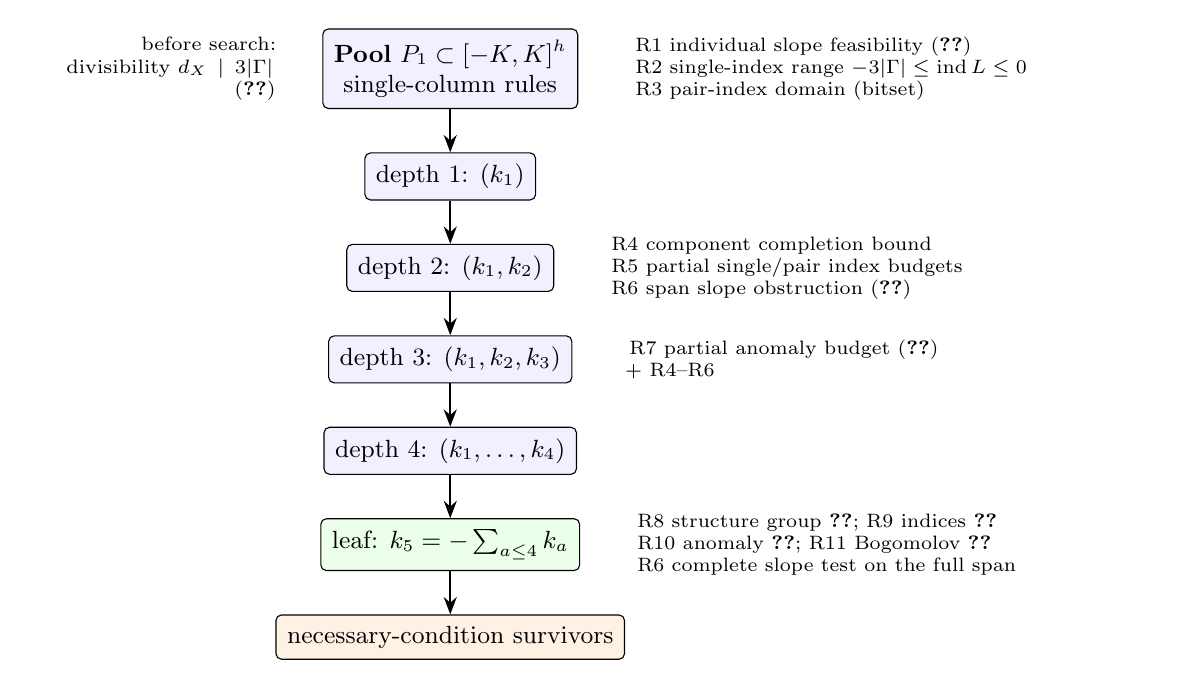
\begin{tikzpicture}[
  node distance=0.55cm and 0.4cm,
  box/.style={draw, rounded corners=2pt, align=center, font=\small, inner sep=4pt, fill=#1},
  box/.default=white,
  rule/.style={font=\scriptsize, align=left, text width=6.6cm},
  arr/.style={-{Stealth[length=2.2mm]}, thick}]
\node[box=blue!6] (pool) {\textbf{Pool} $P_1\subset[-K,K]^h$\\ single-column rules};
\node[box=blue!6, below=of pool] (d1) {depth 1: $(k_1)$};
\node[box=blue!6, below=of d1] (d2) {depth 2: $(k_1,k_2)$};
\node[box=blue!6, below=of d2] (d3) {depth 3: $(k_1,k_2,k_3)$};
\node[box=blue!6, below=of d3] (d4) {depth 4: $(k_1,\dots,k_4)$};
\node[box=green!8, below=of d4] (leaf) {leaf: $k_5=-\sum_{a\le4}k_a$};
\node[box=orange!10, below=of leaf] (surv) {necessary-condition survivors};
\foreach \a/\b in {pool/d1,d1/d2,d2/d3,d3/d4,d4/leaf,leaf/surv} \draw[arr] (\a) -- (\b);
\node[rule, right=0.6cm of pool] {R1 individual slope feasibility (\cref{prop:percoef})\\
  R2 single-index range $-3|\Gam|\le\ind L\le0$\\ R3 pair-index domain (bitset)};
\node[rule, right=0.6cm of d2] {R4 component completion bound\\
  R5 partial single/pair index budgets\\
  R6 span slope obstruction (\cref{prop:monotone})};
\node[rule, right=0.6cm of d3] {R7 partial anomaly budget (\cref{prop:anomalybudget})\\ + R4--R6};
\node[rule, right=0.6cm of leaf] {R8 structure group \ref{c:structure}; R9 indices \ref{c:index}\\
  R10 anomaly \ref{c:anomaly}; R11 Bogomolov \ref{c:bogomolov}\\
  R6 complete slope test on the full span};
\node[rule, left=0.5cm of pool, text width=3.0cm, align=right] {before search:\\ divisibility $d_X\mid3|\Gam|$\\ (\cref{prop:divisibility})};
\end{tikzpicture}
\caption{The search tree. Each rule is a necessary condition (\cref{lem:soundness});
rules R4, R5 and R6 are monotone and prune entire subtrees. Rules R3 and R4 are
enforced by construction through bitset-indexed candidate lists rather than
tested inside the loop.}
\label{fig:tree}
\end{figure}

\subsection{The rules}

\Cref{tab:rules} lists every rule, its status and where it acts. We give the
proofs of those that are not immediate.

\begin{table}[t]
\centering\small
\begin{tabularx}{\textwidth}{@{}lXll@{}}
\toprule
& Rule & Status & Acts at \\
\midrule
R1 & $\mu_k$ has a zero in $T_+$ (signed-matrix test; exact per \cref{prop:percoef}) & exact (bench.) & pool \\
R2 & $-3|\Gam|\le\ind\Oc_X(k)\le0$ (\st{GUT\_FULL}) & necessary & pool \\
R3 & declared domain: $\ind(L_a\otimes L_b)\le0$ for all pairs & domain restriction & pool, prefix \\
R4 & $|\sum_{a\le m}k_a^i|\le(5-m)K$ & necessary & prefix \\
R5 & partial sums of single and pair indices lie in $[-3|\Gam|,0]$ & necessary & prefix \\
R6 & $\spn_\R\{k_a\}\cap P=\{0\}$ (complete slope obstruction) & necessary & prefix, leaf \\
R7 & partial anomaly budget & necessary & prefix \\
R8 & no proper zero-sum subset \ref{c:structure} & exact & leaf \\
R9 & $\ind V=-3|\Gam|$ ($\ind\wedge^2V$ then automatic, \cref{prop:indexidentity}) & exact & leaf \\
R10 & $c_{2,r}-c_2(V)_r\ge0$ & necessary & leaf \\
R11 & Bogomolov pairing & necessary & leaf \\
R12 & $d_X\mid 3|\Gam|$ & exact, unbounded & before search \\
\bottomrule
\end{tabularx}
\caption{Pruning rules. R3 restricts the declared domain to the historical
domain of \cite{ACGLP2013}; it is not claimed necessary, and the independent
replays (\cref{sec:validation}) also run with it removed. R1 is exact on
geometries with $d_{ijj}=0$, which includes both benchmarks.}
\label{tab:rules}
\end{table}

\paragraph{R2 (single-index range).} At a common zero of the slopes, a
nontrivial line bundle $L_a$ has $h^0=h^3=0$, since a line bundle of slope zero
with a nonzero section is trivial, and \ref{c:structure} excludes trivial
summands. No anti-families means $h^2(X,V)=0$, hence $h^2(L_a)=0$ and
$\ind L_a=-h^1(L_a)\le0$. The five indices sum to $-3|\Gam|$, so each lies in
$[-3|\Gam|,0]$, and so does every partial sum (R5).

\paragraph{R4 (component completion).} With $m$ columns fixed, the remaining
$5-m$ columns have entries in $[-K,K]$ and must cancel the partial sum, so
$|\sum_{a\le m}k_a^i|\le(5-m)K$ by the triangle inequality.

\subsection{The slope obstruction}
\label{sec:slope}

Poly-stability of a sum of line bundles with $c_1(V)=0$ means a common zero of
the five slopes:
\begin{equation}\tag{SZ}\label{eq:SZ}
\exists\,t\in T_+:\qquad \mu_{k_a}(t)=t^\top M(k_a)\,t=0\qquad(a=1,\dots,5).
\end{equation}

\begin{lemma}[Sign obstruction]\label{lem:sign}
If $M\in\Sym_h(\Z)$ is nonzero and entrywise nonnegative (or nonpositive), then
$t^\top Mt\neq0$ for every $t\in T_+$.
\end{lemma}
\begin{proof}
Each term $M_{jl}t^jt^l$ has the same weak sign and at least one is strictly
nonzero, because $t^jt^l>0$.
\end{proof}

\begin{proposition}[Combined test]\label{prop:combined}
If \eqref{eq:SZ} holds then for every $c\in\R^5$ the matrix
$M(\sum_ac_ak_a)=\sum_ac_aM(k_a)$ is zero or has entries of both signs.
Contrapositively, a single $c\in\Z^5$ for which $M(\sum_ac_ak_a)$ is nonzero and
one-signed proves that $V$ is not poly-stable anywhere in $T_+$.
\end{proposition}
\begin{proof}
At the witness $t_*$, $t_*^\top M(\sum_ac_ak_a)t_*=\sum_ac_a\mu_{k_a}(t_*)=0$;
apply \cref{lem:sign}.
\end{proof}

The scan of \cite{ACGLP2013} applies \cref{prop:combined} with
$c\in\{-1,0,1\}^5$. This is \emph{sound} but not \emph{complete}: passing the
test for all $c$ in a finite box does not imply \eqref{eq:SZ}. (Since
$\sum_ak_a=0$, $M(\sum_ac_ak_a)$ depends only on the class of $c$ modulo
$\Z(1,\dots,1)$; the 121 vectors of the box with first nonzero entry positive
fall into 106 classes, and the box is exactly the set of classes of spread
$\max c-\min c\le2$.) The quantified statement, however, is decidable exactly.

\begin{proposition}[Exact obstruction cone]\label{prop:cone}
Let $S=\spn_\R\{k_1,\dots,k_5\}\subseteq\R^h$ and
$P=\{k\in\R^h: M(k)_{jl}\ge0\ \forall j,l\}$, a rational polyhedral cone. Some
$c\in\Z^5$ yields a one-signed nonzero combined matrix if and only if $S\cap P$
contains a point $k$ with $M(k)\neq0$.
\end{proposition}
\begin{proof}
$M$ is linear, so $\{M(\sum_ac_ak_a):c\in\R^5\}=M(S)$, and $P$ is the preimage of
the entrywise-nonnegative matrices; $-c$ handles the nonpositive case. A
rational point of the rational cone $S\cap P$ can be scaled to an integer point
$k$, and $c$ is recovered by solving the consistent rational system
$\sum_ac_ak_a=k$, then clearing denominators.
\end{proof}

On geometries with $d_{ijj}=0$ for all $i,j$---both benchmarks---$M(k)$ has zero
diagonal, and nothing is lost per coefficient vector:

\begin{proposition}[Per-coefficient optimality]\label{prop:percoef}
If $d_{ijj}=0$ for all $i,j$, then for any $k\in\Z^h$, the form $\mu_k$ has a
zero in $T_+$ if and only if $M(k)$ is zero or has entries of both signs.
\end{proposition}
\begin{proof}
($\Rightarrow$) is \cref{lem:sign}. ($\Leftarrow$): the diagonal vanishes, so
suppose $M_{jl}>0$ and $M_{j'l'}<0$ at off-diagonal positions. Let $t(T)$ equal
$T$ at positions $j,l$ and $1$ elsewhere; then
$\mu_k(t(T))=2M_{jl}T^2+O(T)\to+\infty$. The analogous path at $(j',l')$ gives
$-\infty$. $T_+$ is connected and $\mu_k$ continuous, so $\mu_k$ vanishes in $T_+$.
\end{proof}

In particular the single-bundle condition ``$\mu(L)=0$ somewhere in the
interior of the Kähler cone'' is decided exactly on these geometries by the
signed-matrix test (R1), and the only incompleteness of the finite test is the
truncation of the $c$-search, which \cref{prop:cone} removes.

\begin{proposition}[Monotonicity]\label{prop:monotone}
If $S'\subseteq S$ and $S'\cap P$ contains a point with $M\ne0$, so does $S\cap P$.
Hence the test applied to the span of any prefix $(k_1,\dots,k_m)$ prunes every
completion of that prefix.
\end{proposition}
\begin{proof}
Immediate from $S'\cap P\subseteq S\cap P$.
\end{proof}

To decide $S\cap P\neq\{0\}$ exactly we need $P$ to be pointed and its extreme
rays.

\begin{lemma}[The tetraquadric cone]\label{lem:rays}
On $\Xa$, $M(k)_{jl}=2(k^m+k^n)$ for $j\ne l$, where $\{m,n\}$ is the
complement of $\{j,l\}$ in $\{1,2,3,4\}$, and $M(k)_{jj}=0$. Hence
$P=\{k\in\R^4:k^m+k^n\ge0\ \forall m<n\}$, $M(k)=0$ only for $k=0$, and $P$ is
pointed with exactly eight extreme rays: the coordinate vectors $e_i$ and the
four vectors with one entry $-1$ and the others $+1$.
\end{lemma}
\begin{proof}
The formula follows from $d_{ijl}=2$ for distinct indices. If all pairwise
sums vanish then $k^1+k^2=k^1+k^3=k^2+k^3=0$ forces $k^1=k^2=k^3=0$ and then
$k^4=0$, so $P\cap(-P)=\{0\}$. A ray of $P$ is extreme iff the constraints tight
on it have rank three. For $e_1$ the tight constraints are the three pairs not
containing $1$; for $(-1,1,1,1)$ the three pairs containing $1$; each set has
rank three. Enumerating the $\binom63=20$ triples of constraints shows there are
no others.
\end{proof}

For $\Xb$ the analogous computation (exact, by enumeration) gives $2h=10$
extreme rays: the $e_i$ and the vectors with one entry $-2=-(h-3)$ and the
others $+1$. In general the implementation enumerates extreme rays of $S\cap P$
exactly in integer arithmetic and declines to prune if the pointedness check
fails.

The primal enumeration costs a number of kernel computations that grows with
the dimension of $S$ and dominated the running time on $\Xb$ (90\% of a profiled
scan). The dual form is much cheaper exactly where the search spends its time.

\begin{proposition}[Dual decision]\label{prop:dual}
Let $P$ be pointed with extreme rays $r_1,\dots,r_s$, let $A$ be a matrix whose
rows span $S^\perp$, and $d=\dim S^\perp=h-\rk S$. Then
\[
S\cap P=\{0\}\iff\exists\,\varphi\in S^\perp:\ \langle\varphi,r_i\rangle>0\ \forall i
\iff 0\notin\conv\{Ar_1,\dots,Ar_s\}\subset\R^d .
\]
\end{proposition}
\begin{proof}
As $P$ is pointed its base $B=\conv\{r_i\}$ is compact with $0\notin B$. If
$S\cap P=\{0\}$ then $S\cap B=\emptyset$, and the compact convex set $B$ is
strictly separated from the closed subspace $S$ by a functional that must vanish
on $S$, i.e.\ lies in $S^\perp$, and is positive on $B$. Conversely such a
$\varphi$ vanishes on $S$ and is positive on $P\setminus\{0\}$. The last
equivalence is Gordan's alternative~\cite{Schrijver1986} for the projected
points $Ar_i$.
\end{proof}

The dimension $d$ \emph{shrinks} as the prefix grows. At the deepest and most
numerous nodes $d\in\{1,2\}$: for $d=1$ the test is whether the projected
scalars take both signs ($O(s)$), for $d=2$ an angular-gap test
($O(s\log s)$). The primal enumeration remains the reference implementation,
the fallback for $d>2$, and the producer of the explicit integer witness $k_c$
recorded in every rejection certificate. The two were differentially tested on
12,000 random column sets across every span rank with no disagreement.

\begin{example}[A spurious survivor of the finite test]\label{ex:spurious}
On $\Xa$ with $\Gam=\Z_2$ at $K=3$, the charge matrix with columns
\[
(-3,-1,1,2),\ (0,1,-1,0),\ (0,1,-1,0),\ (1,1,-1,-1),\ (2,-2,2,-1)
\]
satisfies every other declared condition and passes the test for all
$c\in\{-1,0,1\}^5$; a numerical optimiser stalls at slope residual
$3.6\times10^{-7}$. The complete test rejects it with the integer witness
$k_c=(1,0,0,0)\in S$, for which $M(k_c)$ is entrywise nonnegative and nonzero.
It is absent from the published catalog. Its orbit is the only difference
between the finite and the complete test at $K=3$ (8 versus 7 orbits) and at
$K=4$ (11 versus 10), and removing it is what gives exact catalog agreement
(\cref{sec:validation}).
\end{example}

Soundness was tested by a counterexample search: 12,000 randomly generated
bundles carrying an exact common slope zero on $\Xa$ and $\Xb$ were never
rejected; an independently written Fourier--Motzkin implementation agreed with
the extreme-ray implementation on 3,000 random column sets; and every published
model and every survivor with an exact slope witness is retained.

\subsection{Beyond sign tests: a Pólya hierarchy and an exact decision}
\label{sec:polya}

The sign test is exact per combination only when $d_{ijj}=0$
(\cref{prop:percoef}), and even then a bundle can pass every sign test while its
five slopes have no \emph{simultaneous} zero. Two further exact tools address
this; both produce certificates checked in exact arithmetic.

\begin{proposition}[Pólya certificates]\label{prop:polya}
If for some $c$ and some $N\ge0$ the form
$(t_1+\dots+t_h)^N\sum_ac_a\mu_{k_a}(t)$ has all coefficients nonnegative and not
all zero, then \eqref{eq:SZ} has no solution. Every form strictly positive on the
closed simplex admits such an $N$; $N=0$ is the sign test.
\end{proposition}
\begin{proof}
A nonzero polynomial with nonnegative coefficients is positive on the open
orthant, and $(\sum_it_i)^N>0$ there; at a common zero the combination would
vanish. The converse direction is Pólya's theorem.
\end{proof}

The coefficients are linear in $k_c=\sum_ac_ak_a$, so each level of the hierarchy
is again a polyhedral cone and a certificate is found by linear programming and
verified exactly. On geometries with $d_{ijj}=0$ the hierarchy provably adds
nothing beyond $N=0$ (by \cref{prop:percoef}); on the other catalog geometries we
tested it added no certificate for charges in $[-2,2]$ up to $N=4$. The
obstruction for the bundles below, where it exists, is therefore \emph{joint}.

\begin{proposition}[Exact decision in rank $h-1$]\label{prop:decision}
Suppose $\rk K=h-1$. Set $t_h=1$, which loses no interior point, and compute a
lexicographic Gröbner basis of $h-1$ independent slopes. If it is in shape
position, $t_i=g_i(x)$ and $p(x)=0$; isolate every real root of every irreducible
factor of $p$ in an exact rational interval and enclose the other coordinates by
rigorous interval arithmetic. A root at which all coordinates are positive, and
modulo whose minimal polynomial every slope vanishes identically, is an exact
real-algebraic witness of poly-stability. If no real root is interior, \eqref{eq:SZ}
has no solution.
\end{proposition}
\begin{proof}
In rank $h-1$ the common zeros with $t_h=1$ are the solutions of the $h-1$
independent equations, which in shape position are finitely many and given
exactly by the roots of $p$; interval enclosures that exclude zero decide each
coordinate's sign rigorously.
\end{proof}

When the basis is not in shape position the decision proceeds factor by factor:
factors of $p$ without a positive real root are discarded (an interior point has
$t_{h-1}>0$); a rational root is substituted and the smaller system decided
recursively; over an irrational factor $f$ the remaining coordinates are solved
linearly in $\Q[x]/(f)$ when possible. Anything else, including positive-dimensional
zero sets (rank below $h-1$), is reported as \st{UNDECIDED}. On the tetraquadric the procedure certifies the published model
with witness $t=(1,1,1,1)$, and the spurious candidate of \cref{ex:spurious}, whose
zero set is positive-dimensional, is excluded by the sign test instead: the tools
are complementary.

\subsection{Index identity and divisibility}

\begin{proposition}[Index identity]\label{prop:indexidentity}
On any Calabi--Yau threefold, if $V=\bigoplus_{a=1}^5L_a$ has $c_1(V)=0$ then
$\ind\wedge^2V=\ind V$.
\end{proposition}
\begin{proof}
The linear terms vanish: $\sum_ac_2\cdot k_a=0$ and each $a$ occurs in four
pairs. For the cubic terms,
$\sum_{a<b}D(k_a+k_b)^3=4\sum_aD(k_a)^3+3\sum_{a\ne b}D(k_a,k_a,k_b)$ and
$\sum_{b\ne a}k_b=-k_a$, so the sum is $4\sum_aD(k_a)^3-3\sum_aD(k_a)^3$.
\end{proof}
This is stated in \cite{ACGLP2013} after their equation~(4.7); we use it to
drop a redundant filter and keep it as a free consistency check. (For rank $n$
the coefficient is $n-4$.)

\begin{proposition}[Divisibility obstruction]\label{prop:divisibility}
Let $d_X=\gcd\{\ind\Oc_X(k):k\in\Z^h\}$. If $d_X\nmid3|\Gam|$, no sum of line
bundles on $X$ has $\ind V=-3|\Gam|$, for any charges. Moreover
$d_X=\gcd\{\ind\Oc_X(k):k\in\{0,1,2,3\}^h\}$.
\end{proposition}
\begin{proof}
$\ind V=\sum_a\ind L_a\in d_X\Z$. For the second claim, $\ind$ is an
integer-valued polynomial of degree three, hence a $\Z$-combination of
$\prod_i\binom{k_i}{\alpha_i}$ with $|\alpha|\le3$; its values generate the same
subgroup as the coefficients, which are integer combinations of finite
differences at points of $\{0,1,2,3\}^h$.
\end{proof}

Over the 68 favourable CICYs, $d_X\in\{1,2,3,5\}$ occurs $19,44,4,1$ times.
Combined with the symmetry orders recorded for each geometry, the obstruction
predicts \emph{zero} models for exactly two pairs, $(7761,|\Gam|=2)$ with $d_X=5$
and $(7447,|\Gam|=5)$ with $d_X=2$; the published catalog has zero models for
both, and no catalog entry with models contradicts it. The prediction is not
vacuous: geometries with odd $|\Gam|$ and $d_X\mid3|\Gam|$ do carry models.
The rule is elementary; we have not found it stated in the sources we examined.
It is the only rule here whose conclusion carries no bound on the charges.

\subsection{The partial anomaly budget}

\begin{proposition}\label{prop:anomalybudget}
Assume \ref{c:c1}, a trivial hidden bundle and nef $J_r$. Then \ref{c:anomaly}
implies the separable inequality
\begin{equation}\label{eq:anomaly-separable}
\textstyle\sum_{a=1}^5q_r(k_a)\ \ge\ -2c_{2,r}\qquad\text{for all }r .
\end{equation}
Let $P_1$ be a pool containing every column any valid completion can use, and
$Q_r=\max_{k\in P_1}q_r(k)$. If for a prefix $(k_1,\dots,k_m)$ and some $r$
\[
\textstyle\sum_{a\le m}q_r(k_a)+(5-m)Q_r<-2c_{2,r},
\]
no completion satisfies \eqref{eq:anomaly-separable} and the branch is pruned.
\end{proposition}
\begin{proof}
With $\sum_ak_a=0$ the Whitney formula gives
$c_2(V)_r=-\tfrac12\sum_aq_r(k_a)$, so $c_{2,r}-c_2(V)_r\ge0$ is
\eqref{eq:anomaly-separable}. Each remaining column contributes at most $Q_r$.
\end{proof}

The pool in the implementation is the retained single-column list, itself
defined by necessary conditions, and the derived fifth column is required to
lie in it. The bound is inactive for $K\le2$, since small charges cannot reach
it, and first bites at $K=3$ (\cref{tab:ablation}).

\subsection{Implementation}

Two features matter for the complexity. First, the retained pool is indexed by
bitsets: for each component $i$ and threshold, the set of columns whose
component lies above or below it, and for each column the set of compatible
partners under R3. Rules R3 and R4 are then enforced \emph{by construction}---a
node iterates only over the intersection of the relevant bitsets---rather than
tested inside the loop. This cut fourth-column attempts by factors of 19--28
and wall time by $3$--$7.5\times$ at identical survivor sets, which was
verified by re-running every recorded domain and requiring exact set equality.
Second, the span of the prefix is maintained incrementally in a fraction-free
integer row-reduced form, which is also the memoisation key for the slope
decision, so repeated spans are decided once. Every run is checkpointed; a
checkpoint embeds the SHA-256 of the source and inputs and refuses to resume
under changed code.

\subsection{Measured effect of the pruning}

\Cref{tab:funnel} shows the funnel at $K=2$ and \cref{tab:ablation} the effect
of each rule and of $K$.

\begin{table}[t]
\centering\small
\begin{tabular}{@{}lr@{}}
\toprule
stage ($\Xa$, $\Gam=\Z_2$, $K=2$, finite slope test, pre-indexing engine) & count \\
\midrule
ordered four-column assignments (nominal) & 152,587,890,625 \\
individual columns in the box & 625 \\
retained single columns (R1, R2) & 235 \\
retained depth-2 prefixes & 10,573 \\
retained depth-3 prefixes & 123,629 \\
fourth-column attempts & 7,875,639 \\
retained depth-4 prefixes & 252,154 \\
complete canonical bundles & 38,161 \\
\quad no proper zero-sum subset (R8) & 24,043 \\
\quad $\ind V=-6$ (R9) & 6,261 \\
\quad all pair indices in range (R3) & 1,356 \\
\quad anomaly (R10) & 1,260 \\
\quad slope (R6) & \textbf{120} \\
\bottomrule
\end{tabular}
\caption{Funnel of the search. Prefix counters count prefixes, not full states,
and must not be added as if they partitioned the nominal domain. The ratio of
nominal assignments to materialised bundles, about $4\times10^6$, includes
canonicalisation and is not a pure physics pruning factor; at the last level the
slope obstruction alone removes a factor $10.5$.}
\label{tab:funnel}
\end{table}

\begin{table}[t]
\centering\small
\begin{tabular}{@{}rlrrrrrr@{}}
\toprule
$K$ & slope rule & wall (s) & RSS (MiB) & 4th-col.\ attempts & bundles built & survivors & orbits \\
\midrule
1 & finite & 0.05 & 25.4 & 4,636 & 713 & 0 & 0 \\
1 & complete & 0.09 & 25.3 & 2,535 & 334 & 0 & 0 \\
2 & finite & 4.00 & 33.2 & 420,266 & 38,161 & 120 & 5 \\
2 & complete & 3.99 & 37.2 & 170,121 & 10,097 & 120 & 5 \\
3 & finite & 15.88 & 50.5 & 2,304,135 & 146,425 & 192 & \textbf{8} \\
3 & complete & 18.42 & 68.3 & 963,549 & 52,800 & 168 & 7 \\
4 & finite & 36.65 & 65.6 & 7,147,830 & 294,130 & 264 & \textbf{11} \\
4 & complete & 43.62 & 105.6 & 3,236,246 & 118,577 & 240 & 10 \\
5 & complete & 85.44 & 141.0 & 6,537,468 & 162,761 & 240 & 10 \\
6 & complete & 118.88 & 193.8 & 10,199,673 & 206,847 & 240 & 10 \\
7 & complete & 179.15 & 188.9 & 14,516,351 & 231,946 & 240 & 10 \\
\bottomrule
\end{tabular}
\caption{$\Xa$, $\Gam=\Z_2$, target \st{GUT\_FULL}, bitset-indexed engine.
Orbits are ambient-row orbits of the column-canonical survivors. The finite test
retains one spurious orbit at $K=3$ and $K=4$ (\cref{ex:spurious}). With the dual
decision of \cref{prop:dual} the complete rule at $K=4$ takes 28.8\,s, faster
than the finite test. The partial anomaly budget (\cref{prop:anomalybudget})
first acts at $K=3$, pruning 3,734 depth-3 and 166,040 depth-4 branches under the
complete rule and reducing built bundles from 75,534 to 52,800.}
\label{tab:ablation}
\end{table}

Two observations. The complete slope rule, applied at every depth, removes
2,730 of the 10,573 depth-2 prefixes already at $K=2$, and cuts the bundles
built by factors of $2.8$ at $K=3$ and $2.5$ at $K=4$. And the pruning improves
with $K$ rather than degrading: from $K=1$ to $3$ the nominal domain grows by
factors $3,544$ and $218$ while the bundles built grow by $30$ and $5.2$.

\section{Searches with no charge cutoff}
\label{sec:slices}

A box search says nothing about charges outside the box. This section shows
that for an explicit and large part of the landscape the box can be removed
altogether.

\subsection{The slice decomposition}

Write $q_i(t)=d_{ijl}t^jt^l$, so that $\mu_{k}(t)=\langle k,q(t)\rangle$.

\begin{proposition}[Slices]\label{prop:S1}
Suppose $q_i(t)>0$ on $T_+$ for every $i$ (on both benchmarks
$q_i(t)=4e_2(t_{\neq i})$). If $V=\bigoplus_aL_a$ satisfies \eqref{eq:SZ}, there is
a primitive $p\in\Z^h$ with every $p_i>0$ such that $\langle k_a,p\rangle=0$ for
all $a$.
\end{proposition}
\begin{proof}
At a witness $t$, $u=q(t)\in\R^h_{>0}$ and $\langle k_a,u\rangle=\mu_{k_a}(t)=0$,
so $u\in S^\perp$ with $S=\spn_\R\{k_a\}$. $S$ is spanned by integer vectors, so
$S^\perp$ is a rational subspace; it meets the open positive orthant (at $u$),
and rational points are dense in it, so it contains a positive rational vector.
Clear denominators and divide by the gcd.
\end{proof}

\begin{corollary}
$\rk K\le h-1$ for every slope-feasible charge matrix. (Confirmed on data: all
240 $\Xa$ survivors at $K\le7$ have rank 3 or 2, never 4.)
\end{corollary}

The decomposition is exhaustive: every slope-feasible model lies in the slice
$p^\perp$ of at least one positive primitive $p$. One search over
$\Z^{h\times5}$ becomes a family of searches over rank-$(h-1)$ lattices.

\subsection{A charge bound on good slices}

Summing \eqref{eq:anomaly-separable} over $r$ gives, with $s(k)=\sum_ik^i$,
\begin{equation}\label{eq:CX}
\sum_{a=1}^5F(k_a)\le C_X,\qquad F(k)=|k|^2-s(k)^2,\qquad
C_X=\frac{\sum_rc_{2,r}}{h-2},
\end{equation}
because on both benchmarks $\sum_rq_r(k)=2(h-2)\bigl(s(k)^2-|k|^2\bigr)$; hence
$C_X=48$ for $\Xa$ and $40$ for $\Xb$.

\begin{proposition}[Per-slice bound]\label{prop:S2}
Let $p$ be a slice direction with
\begin{equation}\label{eq:star}
\Bigl(\sum_ip_i\Bigr)^2>(h-1)\,|p|^2 .
\end{equation}
Then $F$ is positive definite on $p^\perp$, and every column of every model in
the slice satisfies
\[
|k_a|^2\ \le\ R^2(p)\coloneqq\frac{C_X\,|p|^2}{(\sum_ip_i)^2-(h-1)|p|^2}.
\]
\end{proposition}
\begin{proof}
For $k\in p^\perp$ let $w$ be the orthogonal projection of $\mathbf 1=(1,\dots,1)$
onto $p^\perp$. Then $s(k)=\langle k,w\rangle$, so $s(k)^2\le|k|^2|w|^2$ and
$F(k)\ge|k|^2(1-|w|^2)$. Since $|w|^2=h-(\sum p)^2/|p|^2$, condition \eqref{eq:star}
is exactly $|w|<1$. Every summand in \eqref{eq:CX} is then nonnegative, hence
bounded by $C_X$, and $|k_a|^2(1-|w|^2)\le C_X$.
\end{proof}

\begin{corollary}[A search with no charge cutoff]
For $p$ satisfying \eqref{eq:star} the admissible column pool
$P(p)=\{k\in\Z^h:\langle k,p\rangle=0,\ F(k)\le C_X\}$ is finite and exactly
computable, by walking the ball $|k|^2\le R^2(p)$ and solving the linear
condition for the last coordinate. Searching $P(p)$ with the rules of
\cref{sec:search} exhausts the entire slice over all integer charges. The outcome
\st{UNSAT\_SLICE\_UNBOUNDED} carries no charge bound.
\end{corollary}

\subsection{Results on the tetraquadric}

On $\Xa$ with $\Gam=\Z_2$ and target \st{GUT\_FULL}, of the primitive positive
$p$ with entries $\le10$ (up to permutations of the ambient factors), 469 satisfy
\eqref{eq:star}. All were exhausted in 36.7\,s in total:

\begin{center}
\small
\begin{tabular}{@{}lr@{}}
\toprule
slices satisfying \eqref{eq:star}, entries $\le10$ & 469 \\
\quad proven empty for all charges (\st{UNSAT\_SLICE\_UNBOUNDED}) & \textbf{425} \\
\quad containing models & 44 \\
\qquad ambient-row orbits found, maximum charge & 6 orbits, $\max|k|=3$ \\
largest radius $R^2(p)$ & 2,484 \\
column pool sizes & 85--700 \\
\bottomrule
\end{tabular}
\end{center}

Pools stay small although radii grow, because the lattice $p^\perp$ thins as $|p|$
grows.

\subsection{Where the difficulty is}

The slices that fail \eqref{eq:star} are not an artefact of the method: real
models live there. For $p=(1,1,3,4)$, $(\sum p)^2=3|p|^2$ exactly, and
$p=(1,1,4,4)$ has $100<102=3|p|^2$. There $F$ is degenerate or indefinite on
$p^\perp$, the pool is genuinely infinite, and the anomaly bounds nothing. What
stops the charges on these slices is the \emph{index}, which grows cubically
along the directions with $F\le0$: on the null ray of $p=(1,1,3,4)$, $\ind$ takes
the values $2,52,198$ at $k=(-2,-2,0,1),(-4,-4,0,2),(-6,-6,0,3)$, leaving the
window $[-3|\Gam|,0]$ at once. More generally $F(k)\le0$ forces $s(k)\ne0$ (if
$s(k)=0$ then $F(k)=|k|^2>0$), so on $\Xa$
$\ind(nk)=2\bigl(n^3e_3(k)+n\,s(k)\bigr)$ is unbounded along every such ray.
Converting this ray-wise statement into a bound on the semialgebraic set
$\{F\le0,\ \ind\in[-3|\Gam|,0]\}$ is the open step; we state it as a problem in
\cref{sec:limitations}.

Probing the 22 uncovered slices with entries $\le6$ at an in-slice box $K=16$,
far beyond the full-box reach, over pools with thousands of large-charge
columns, produces maximum charge 4 and nothing new. The 84 proven slices with
entries $\le6$ together with these 22 probed ones reproduce \emph{exactly} the
10 orbits of the full $K=7$ search and of the published catalog.

\subsection{A conditional bound}

\begin{conjecture}[Charge bound from anomaly and slope]\label{conj:C1}
Writing $u=q(t)$ for a slope witness and
$\delta(u)^2=h-(\sum_iu_i)^2/|u|^2$, the argument of \cref{prop:S2} gives
$\sum_a|k_a|^2\bigl(1-\delta(u)^2\bigr)\le C_X$, a bound whenever $\delta(u)<1$.
On $\Xa$ the infimum of $(\sum u)^2/|u|^2$ over the attainable $u$ is exactly 3,
approached as one $t_i\to0$, so $\delta\to1$ and the bound degenerates near the
boundary of the Kähler cone. We conjecture that the index condition keeps slope
witnesses of index-admissible models uniformly away from that boundary, which
would make the set of models on $\Xa$ finite by this route.
\end{conjecture}

We make no finiteness claim. Finiteness of the \emph{topology} of
$V$ is argued in~\cite{ACGLP2013}; the conjecture concerns the charges
themselves.

\section{Certified line-bundle cohomology}
\label{sec:cohomology}

The spectrum condition \ref{c:spectrum} needs $h^q(X,L)$ for the line bundles
$L_a$ and $L_a\otimes L_b$. We compute these from the Koszul resolution of
$\Oc_X$ in $A$~\cite{Hubsch1992,AGHL2010},
\[
E_1^{-p,q}=H^q\bigl(A,\ L\otimes\wedge^pN^*\bigr)\ \Longrightarrow\ H^{q-p}(X,L),
\]
where each $E_1$ term is the cohomology of a line bundle on a product of
projective spaces, given by Bott's formula~\cite{Bott1957} and Künneth. (Closed
formulae are known for several CICYs~\cite{CL2018}, and the map ranks of these
Koszul complexes have been studied through Hilbert functions~\cite{Wang2026}; we
use neither as input, only the exact spectral sequence.)

\paragraph{Collapse.} The differential $d_r$ has bidegree $(r,1-r)$. If no
differential can join two occupied $E_1$ nodes, the sequence degenerates at
$E_1$ and each $h^q(X,L)$ is read off. This bidegree-support test is exact.

\paragraph{One differential.} When exactly two nodes are occupied and joined by
one differential $\Phi$, the cohomology is $\ker\Phi$ and $\operatorname{coker}\Phi$.
$\Phi$ is induced by the defining equations, so in the fixed monomial bases of
the ambient cohomology it is a matrix $\Phi(c)$ whose entries are $\Z$-linear in
the coefficient vector $c$ of the equations.

\begin{proposition}[Generic rank from one finite-field minor]\label{prop:rank}
Let $\Phi(c)\in\mathrm{Mat}_{m\times n}(\Z[c])$ with entries polynomial in $c$,
let $c_0\in\Z^N$, $p$ a prime, and suppose $\rk_{\F_p}\bigl(\Phi(c_0)\bmod p\bigr)\ge r$.
Then (i) some $r\times r$ minor $\delta\in\Z[c]$ has $\delta(c_0)\ne0$, so
$\delta\ne0$; (ii) $\rk\Phi(c)\ge r$ on the nonempty Zariski-open set
$\{\delta\ne0\}$, over $\Q$ and $\C$; (iii) if $r=\min(m,n)$ the generic rank is
maximal.
\end{proposition}
\begin{proof}
A matrix over a field has rank $\ge r$ iff some $r\times r$ minor is nonzero,
and taking minors commutes with reduction $\Z\to\F_p$, so the nonzero minor mod
$p$ is the reduction of an integer $\delta(c_0)\ne0$. A polynomial with a nonzero
value is nonzero, and the coefficient space is irreducible, so
$\{\delta\ne0\}$ is dense open; (iii) adds the bound $\rk\le\min(m,n)$.
\end{proof}

No good-reduction hypothesis is needed: the certificate uses only
``nonzero mod $p$ $\Rightarrow$ nonzero in $\Z$'', never the converse, since
reduction can only lower rank. The prime is unconstrained and $c_0$ need not
even lie in the smooth locus. Failure mod $p$ is inconclusive and is reported as
\st{UNKNOWN}, never as a rank deficiency. Finitely many such certificates hold
simultaneously on a dense open set of smooth members, because the coefficient
space is irreducible. Every certificate records $c_0$, $p$, the matrix
dimensions and a hash of the matrix, and is replayed by the test suite; the
resulting $h^q$ must also satisfy the exact index~\eqref{eq:hrr} and Serre
duality, which are independent postconditions.

\begin{remark}[Scope]
The certified dimensions hold for the \emph{generic} member of the smooth
family with the given configuration. They do not establish the cohomology of a
particular member---in particular of a member admitting a chosen free action,
whose equations lie in a proper closed subfamily---on which dimensions can jump.
For the downstairs analysis we therefore redo the rank computations on a
generic member \emph{of the invariant family} (\cref{sec:equivariant}).
\end{remark}

\paragraph{Reproduction.} For the published $\Xb$ model of~\cite{ACGLP2013}
the engine reproduces $c_1=0$, $\ind V=\ind\wedge^2V=-12$, $c_2(TX)=c_2(V)$, an
exact rational slope witness $t=(5,29,15,11,5)$, and the generic cohomology
$h^\bullet(V)=(0,12,0,0)$, $h^\bullet(\wedge^2V)=(0,15,3,0)$, with every nontrivial
rank certified by \cref{prop:rank}. Poly-stability witnesses in general are
certified exactly: rational $t$ found by lattice search, or real-algebraic $t$
certified by isolating a root and bounding the remaining slopes with rational
interval arithmetic; numerical witnesses are recorded as
\st{NUMERIC\_WITNESS} and never accepted.

\section{Validation: independent replay and exact catalog agreement}
\label{sec:validation}

Two kinds of evidence support the searches: an independent implementation that
exhausts complete domains without sharing any search logic, and model-for-model
agreement with the published catalogs.

\subsection{Independent exhaustive replay}

A standalone enumerator hard-codes the published topology, re-implements HRR,
the subset criterion, the anomaly pairing and the slope obstruction---the latter
by Fourier--Motzkin elimination rather than extreme rays---and visits every
ordered four-column assignment of the domain, deriving the fifth column,
canonicalising, and applying the declared conditions to each distinct class.

\begin{table}[h]
\centering\footnotesize
\setlength{\tabcolsep}{3.5pt}
\begin{tabular}{@{}llrrrrl@{}}
\toprule
geometry & domain & ordered states & valid 5th col. & canonical & surv. & set equality \\
\midrule
$\Xa$, $K=1$ & \st{GUT\_FULL}, pairs $\le0$ & 43,046,721 & 6,765,201 & 58,781 & 0 & exact \\
$\Xa$, $K=1$ & \st{GUT\_FULL}, pairs free & 43,046,721 & 6,765,201 & 58,781 & 0 & exact \\
$\Xa$, $K=1$ & \st{GUT\_CHIRAL}, pairs free & 43,046,721 & 6,765,201 & 58,781 & 0 & exact \\
$\Xb$, $K=1$ & \st{GUT\_FULL}, pairs $\le0$ & 3,486,784,401 & 345,025,251 & 2,906,223 & 0 & exact \\
\bottomrule
\end{tabular}
\caption{Independent replays. The valid-fifth-column counts equal $51^4$ and
$51^5$, matching a closed form (51 of the 81 four-tuples per component have sum
in $[-1,1]$), an arithmetic check on the enumeration itself. The $\Xb$ replay
took 2,434\,s at 783\,MiB.}
\label{tab:replay}
\end{table}

The replay census also shows which condition is load-bearing. On $\Xa$, of the
58,781 canonical states 38,784 pass the subset criterion and 1,932 have the
right index; with unrestricted pair indices all 1,932 pass the anomaly pairing
and \emph{all} are eliminated by the slope obstruction and by nothing else. On
$\Xb$ the funnel is $2{,}906{,}223\to2{,}477{,}960\to132{,}870\to44{,}580\to2{,}040$,
and again all 2,040 anomaly survivors fall to the slope obstruction. This is why
the slope rule's soundness and completeness (\cref{sec:slope}) matter. The
census also confirms $\ind V=\ind\wedge^2V$ on all 58,781 $\Xa$ states, with both
always even ($d_X=2$).

\subsection{Exact agreement with the published catalogs}

We compare row orbits: survivor sets are canonicalised under summand
permutations and permutations of identical ambient factors, and nothing else
(dualisation is not an equivalence, as it flips $\ind V$). The published catalog
is restricted to the same box. The published database does not state a box per
geometry, so ``inside the box'' is our restriction.

\begin{table}[h]
\centering\footnotesize
\setlength{\tabcolsep}{4pt}
\begin{tabular}{@{}llrrrl@{}}
\toprule
geometry, $|\Gam|$ & $K$ & published & ours, finite test & ours, complete test & set equality \\
\midrule
$\Xa$, 2 & 2 & 5 & 5 & 5 & exact \\
$\Xa$, 2 & 3 & 7 & 8 & 7 & exact (complete) \\
$\Xa$, 2 & 4--7 & 10 & 11 (at $K=4$) & 10 & exact, full catalog \\
$\Xa$, 4 & 5 & 58 & -- & 58 & exact, full catalog \\
$\Xb$, 2 & 1 & 0 & -- & 0 & exact \\
$\Xb$, 2 & 2 & 56 & -- & 56 & exact, predicted \\
$\Xb$, 2 & 3 & 87 & -- & 87 & exact, predicted \\
$\Xb$, 2 & 4 & 93 & -- & 93 & exact, full catalog, predicted \\
\bottomrule
\end{tabular}
\caption{Row-orbit comparison with the published GUT catalog~\cite{ACGLP2013,OxfordCICY}.
``Exact'' means 0 published-only and 0 ours-only orbits. The $\Xb$ counts were
predicted from the published $\max|k|$ distribution before each run.}
\label{tab:catalog}
\end{table}

Three points deserve emphasis. First, agreement is \emph{set} equality, not
count agreement: an earlier count agreement with Table~4 of \cite{ACGLP2013} at
$K=2$ was upgraded to catalog identity only after retrieving and parsing the
database itself (63,325 models on 68 geometries, reproducing the counts stated
by its authors). Second, our survivor sets are necessary-condition survivors
while the catalog is the poly-stable, anomaly-free, correct-index stage, so
agreement means the two condition sets coincide \emph{on these domains}; it is
not a proof that our conditions are sufficient in general. Third, the finite
slope test fails to reach agreement at $K=3$ and $K=4$ because of the single
spurious orbit of \cref{ex:spurious}.

Every one of the 10 published $\{\Xa,2\}$ models, the 58 $\{\Xa,4\}$ models and
the 93 $\{\Xb,2\}$ models passes every exact necessary check we implement,
including the complete slope obstruction, as soundness requires.

\subsection{All 68 favourable CICYs}
\label{sec:survey}

To test the engine beyond the two benchmarks we ran it, unchanged, on every
(geometry, $|\Gam|$) key of the published GUT catalog: $K=1$ on all 110 keys
(all 68 geometries, $h^{1,1}\le6$), $K=2$ on the 101 keys with $h^{1,1}\le5$ and
$K=3$ on the 60 keys with $h^{1,1}\le4$, 271 runs in total, each recording the
statistics of \cref{tab:ablation}. Orbits
are taken under summand permutations and under ambient-factor permutations that
preserve the configuration matrix up to a relabelling of its columns.

\begin{table}[h]
\centering\small
\begin{tabular}{@{}rlrrrrrr@{}}
\toprule
$K$ & $h^{1,1}$ & keys & geometries & exact & published in box & recovered & extra orbits \\
\midrule
1 & 2--6 & 110 & 68 & 109 & 40 & \textbf{40} & 1 \\
2 & 2--5 & 101 & 60 & 91 & 9,016 & \textbf{9,016} & 79 \\
3 & 2--4 & 60 & 37 & 60 & 342 & \textbf{342} & 0 \\
\bottomrule
\end{tabular}
\caption{The engine on the whole published catalog. The longest run ($\Xb$ with
$|\Gam|=20$, $K=2$) took 8,794\,s and 947\,MiB; every $h^{1,1}=6$ run at $K=1$
finished within 484\,s.}
\label{tab:survey}
\end{table}

\textbf{No published model inside a box is ever missed}, on any geometry, and the
divisibility obstruction fires on exactly the keys where the catalog is empty.
Our survivor set is a necessary-condition set, and on eleven runs (none of them at
$K=3$) it contains extra orbits---80 in total, ten of the eleven runs on geometries with
$d_{ijj}\neq0$, where the sign test is not exact (\cref{prop:percoef}). Each extra
was classified with the tools of \cref{sec:polya}:

\begin{center}\small
\begin{tabular}{@{}lr@{}}
\toprule
certified unstable (exact decision, \cref{prop:decision}) & 53 \\
certified \emph{stable} (exact real-algebraic witness) & 9 \\
numerically unstable (charge-matrix rank $<h-1$; not a proof) & 18 \\
\bottomrule
\end{tabular}
\end{center}

The 53 are false survivors of the necessary conditions, now excluded exactly;
the 18 are very probably the same, but only numerically. Before trusting
``certified unstable'' we ran the decision on 548 published models, which are
poly-stable and must never be rejected: a first implementation rejected 91 of
them, which exposed two bugs (a positive root whose isolating interval began at
zero was discarded; a polynomial remainder was taken in the wrong order); after
fixing both, it rejects none and certifies 214 of them stable with exact
witnesses. The check is part of the test suite.

\paragraph{A GUT model missing from the catalog.} The nine certified-stable
extras are a single model: they share one full triple-intersection fingerprint
$\{D(k_a,k_b,k_c),\,c_2\cdot k_a\}$ up to summand permutation, invariant under any
automorphism of the Picard lattice preserving $d_{ijk}$, across CICYs 5256, 5301
and 5452, which the catalog records as descriptions of one manifold. On CICY 5256
with $|\Gam|=4$ its charge vectors are
\[
(-2,0,-1,1,0),\ (0,-1,1,-2,1),\ (0,2,1,0,-1),\ (1,-2,1,0,0),\ (1,1,-2,1,0).
\]
It satisfies $c_1(V)=0$, the structure-group criterion, $\ind V=\ind\wedge^2V=-12$,
the anomaly and Bogomolov conditions, and it is poly-stable: with $t_5=1$, $t_4$ is
the unique root in
\[
t_4\in\left[\tfrac{642595}{64736},\ \tfrac{769226}{77493}\right]
\]
of an irreducible degree-12 integer polynomial, the remaining coordinates are
polynomials in $t_4$ proved positive by interval arithmetic, and all five slopes
vanish identically modulo that polynomial. The Kähler class has $t_{\max}/t_{\min}\approx231$. The published
catalog lists 2,128 models on this key with charges up to $|k|=6$, 656 of them in
the box $|k|\le2$ that contains this model, and none with its fingerprint. The
model therefore satisfies every condition the catalog states and is absent from
it. We do not know why; a stability search confined to moderate Kähler ratios
would miss it. It does not descend with individually equivariant line bundles
under any of the four free $\Z_2\times\Z_2$ actions on this manifold, so it is a
new GUT model rather than a new standard model.

\paragraph{Empirical saturation.} On $\Xa$ with $\Gam=\Z_2$ the survivor set is
literally identical at $K=4,5,6,7$, and no survivor uses a charge above 4. We
record this as \st{EMPIRICAL\_SATURATION} at $K=4$. It is not a theorem and no
unbounded inference is drawn from it; the slice results of \cref{sec:slices}
are the unbounded statements we can actually prove.

\paragraph{Topology.} Recomputing $c_2(TX)$ and the Euler number from the
configuration matrices of all 68 favourable CICYs in the catalog reproduces the
published values in 68/68 cases each.

\section{The $\Gam$-representation on cohomology from first principles}
\label{sec:equivariant}

Which states survive the quotient $X\to X/\Gam$ is decided by the
$\Gam$-representation on $H^q(X,L)$. Published databases supply these
representations as data. To search rather than verify, we compute them from the
explicit group action: generators acting linearly on the ambient coordinates,
together with their action on the defining polynomials, both taken from the
published symmetry data~\cite{Braun2011,OxfordCICY}.

\subsection{Characters from the Koszul resolution}

The Koszul resolution is $\Gam$-equivariant, so in the representation ring
\begin{equation}\label{eq:equivariant-koszul}
\sum_q(-1)^q\bigl[H^q(X,L)\bigr]=\sum_p(-1)^p\sum_q(-1)^q\bigl[H^q(A,L\otimes\wedge^pN^*)\bigr].
\end{equation}
Each term on the right is elementary. On a factor $\PP^n$ on which a group element
acts by $M$, let $h_m$ be the complete homogeneous symmetric function of the
eigenvalues of $M$, computed from the characteristic polynomial by Newton's
recursion $h_m=\sum_{i\ge1}(-1)^{i-1}e_ih_{m-i}$ without extracting eigenvalues.
By Bott's theorem and Serre duality
\[
\tr\bigl|_{H^0(\PP^n,\Oc(m))}=h_m\ (m\ge0),\qquad
\tr\bigl|_{H^n(\PP^n,\Oc(m))}=\det(M)^{m+n}\,h_{-m-n-1}\ (m\le-n-1),
\]
and zero otherwise~\cite{Hartshorne1977}; Künneth multiplies over factors. The normal bundle carries
the action $\rho$ on the defining polynomials: grouping the polynomials by
multidegree, the trace on $\wedge^pN^*$ is a product of elementary symmetric
functions $e_{p_c}(\rho_c^{-1})$ over the groups. (Ignoring $\rho$ is correct only
for invariant polynomials, which most geometries do not have.) For abelian
$\Gam$ the multiplicity of a character $\chi$ is the finite Fourier transform
$|\Gam|^{-1}\sum_g\operatorname{char}(g)\overline{\chi(g)}$~\cite{Serre1977}.
All arithmetic is exact over cyclotomic fields.

\subsection{Separating the degrees}

\eqref{eq:equivariant-koszul} gives only the alternating sum. This suffices for
the \emph{chiral} content, $H^1-H^2$, but not for vector-like pairs: $H^1$ and
$H^2$ of a pair bundle can be isomorphic as representations and cancel. Two
mechanisms separate the degrees.

\begin{itemize}[leftmargin=*]
\item \emph{Collapse.} When the bidegree-support test of \cref{sec:cohomology}
  shows the Koszul sequence degenerates at $E_1$, each $H^q(X,L)$ is the sum of
  the $E_1$ characters with $q-p$ equal to that degree.
\item \emph{Equivariant map ranks.} Otherwise, when one differential joins two
  nodes, it is multiplication by the defining polynomial $f$. For $f$ in the
  invariant family the differential is $\Gam$-equivariant, so it preserves
  isotypic components and its rank splits character by character; kernel and
  cokernel per character give both surviving degrees.
\end{itemize}

The second mechanism needs the action matrices themselves. On a $\PP^1$ factor
with block $B$, the action on $H^0(\Oc(m))$ is $\Sym^m(B)$ and on
$H^1(\Oc(m))$ it is $\det(B)^{-1}\bigl(\Sym^{-m-2}(B)\bigr)^{-\top}$ by Serre
duality; Künneth gives Kronecker products. Their traces agree with the
symmetric-function characters---two independent computations of the same
numbers---and the equivariance $\Phi\,\rho_{\mathrm{src}}(g)=\rho_{\mathrm{tgt}}(g)\,\Phi$
is \emph{verified} for every element rather than assumed, which tests the action
matrices, the parsing of the invariant polynomials and the basis conventions at
once. For groups of exponent two all characters are $\pm1$ and all matrices
rational, and the ranks are computed exactly over $\Q$; this makes the largest
bundles tractable (ambient dimension 120 in under a second) and agrees with the
symbolic computation wherever both were run.

\subsection{An equivariance obstruction}

\begin{proposition}\label{prop:equivariance}
Let $G\subset GL$ be the matrix group generated by a lift of $\Gam$ to the
ambient coordinates, a central extension of $\Gam$. Then $\Oc_X(k)$ admits a
$\Gam$-equivariant structure compatible with this lift if and only if every
central element of $G$ that acts trivially on $A$ acts trivially on
$\Oc_A(k)$. For the $\Z_2\times\Z_2$ action on $\Xa$ the two generators do not
commute in $GL_8$: their commutator is $-1$ on every $\PP^1$ factor, which is
trivial on $A$ but acts on $\Oc(k)$ by $(-1)^{\sum_ik^i}$. Hence $\Oc_X(k)$ is
equivariant exactly when $\sum_ik^i$ is even.
\end{proposition}

This is checked, not assumed; when it fails the cohomology carries only a
projective representation and the computation refuses. A second, independent
safeguard rejects any character function whose decomposition is not by
nonnegative integers.

\subsection{Validation}

The published database lists the character tables of every relevant cohomology
group. Comparing all four degrees of every table over the 13 geometries that
carry downstairs models:

\begin{center}\small
\begin{tabular}{@{}lr@{}}
\toprule
models & 2,012 \\
character tables compared (9,181 single, 18,640 pair; all degrees) & 27,821 \\
\textbf{exact agreement} & \textbf{27,821} \\
\bottomrule
\end{tabular}
\end{center}

One convention had to be identified. The published tables are the \emph{raw}
characters of the lift, and the equivariant structure---$\chi_a$ for $L_a$,
$\chi_a+\chi_b$ for $L_aL_b$---is applied only when the downstairs spectrum is
formed; that step is load-bearing, since with it 1,948 of 1,948 published charged
spectra are reproduced exactly and without it only 1,503. Only tables that are
not invariant under their shift distinguish ``raw'' from ``shifted''. There are
694 such tables, all vector-like pair bundles, and all 694 match the raw
computation while none matches the shifted one. (An earlier version of our
comparison applied the shift to the computed side and reported these 694 as
unexplained relabellings; the discrepancy was ours.) A further 640 published pair
entries are unevaluated rank expressions and are not compared. Two genuine bugs
were found by this comparison: CICY 7487 carries four distinct free
$\Z_2\times\Z_2$ actions and each model must use its own, and the polynomial twist
$\rho$ cannot be ignored.

End to end, all 22 published downstairs models on $\Xa$ have their complete
charged spectrum---chiral and vector-like---derived from first principles and
matching the published spectra; every non-collapsing pair bundle involved (21
occurrences of 5 distinct bundles) is resolved by equivariant ranks. The Wilson-line projection itself is exact
bookkeeping (\cref{sec:downstairs}), and against the whole database, with the
published characters as input, it reproduces 1,948 of 1,948 complete records.

\section{A downstairs search on the tetraquadric quotient}
\label{sec:downstairs}

\subsection{Wilson lines and equivariant structures}

For abelian $\Gam$ the Wilson line is a pair of characters: $\chi_T$ on the colour
triplet and $\chi_D$ on the weak doublet of the fundamental $\five$. Everything
else follows from $\ten=\wedge^2\five$:

\begin{center}\small
\begin{tabular}{@{}llll@{}}
\toprule
multiplet & pieces & Wilson-line character & $6Y$ \\
\midrule
$\ten$ & $Q$, $u^c$, $e^c$ & $\chi_T\chi_D$, $\chi_T^2$, $\chi_D^2$ & $1,-4,6$ \\
$\bfive$ & $d^c$, $L$ & $\chi_T^{-1}$, $\chi_D^{-1}$ & $2,-3$ \\
\bottomrule
\end{tabular}
\end{center}

\begin{lemma}\label{lem:wilson}
The Wilson line lies in $SU(5)$, so $\chi_T^3\chi_D^2=1$. For a group of exponent
two this forces $\chi_T=1$ and leaves $\chi_D$ free.
\end{lemma}

A piece with Wilson-line character $\chi$ on a bundle with equivariant structure
$e$ survives with the multiplicity of the upstairs character $\chi-e$ (in
additive notation). Equivariant structures are enumerated subject to
$\sum_ae_a=0$, so that $\det V$ descends. The Wilson line is thus derived, not
chosen; for $\Xa/(\Z_2\times\Z_2)$ it reproduces the convention of the published
database.

\subsection{Results}

Starting from the 58 ambient-row orbits of our exhaustive $\Gam=\Z_2\times\Z_2$,
$K=5$ scan of $\Xa$, with no published input beyond the symmetry data:

\begin{center}\small
\begin{tabular}{@{}lr@{}}
\toprule
upstairs orbits examined & 58 \\
\quad some $L_a$ not equivariant ($\sum_ik^i$ odd, \cref{prop:equivariance}) & 26 \\
\quad equivariant, all needed cohomology determined & 32 \\
\qquad no Wilson line and equivariant structure gives an acceptable spectrum & 11 \\
\qquad \textbf{three chiral families, no charged chiral exotics, a Higgs pair} & \textbf{21} \\
\bottomrule
\end{tabular}
\end{center}

All 10 orbits of the published standard-model database on this quotient are
recovered. The other 11 are absent from it. We call them \emph{candidates} and
label them A01--A11.

\subsection{Audit of the eleven candidates}

Each candidate was frozen into an immutable manifest and audited against every
condition of the original construction:

\begin{center}\small
\begin{tabular}{@{}lr@{}}
\toprule
condition & result \\
\midrule
$c_1(V)=0$, structure group, anomaly, Bogomolov & 11/11 \\
poly-stability with an \emph{exact} witness & 11/11 (8 rational, 3 real-algebraic) \\
$\ind V=\ind\wedge^2V=-12$ & 11/11 \\
$h^\bullet(V)=(0,12,0,0)$, $h^\bullet(\wedge^2V)=(0,12+n_h,n_h,0)$, $n_h>0$ & 11/11 \\
every bundle equivariant; all character tables determined & 11/11 \\
three $Q,u^c,d^c,L,e^c$; no charged chiral exotics; a Higgs pair & 11/11 \\
no colour-triplet Higgs & 11/11 \\
absent from every published downstairs model & 11/11 \\
\bottomrule
\end{tabular}
\end{center}

For charge matrices of rank two the slope-zero locus is a curve, so rationalising
a numerical point cannot produce an exact witness; a rational point \emph{on}
the curve is found instead (for A02, $t=(15,15,3,1)$). Two of the real-algebraic
witnesses have $t_1=4+\sqrt{21}$.

\subsection{Why the candidates are absent from the published database}

The published standard-model database was built from a GUT scan over
$-3\le k_a^i\le3$ on $h^{1,1}=4$ \cite[Sec.~5.3]{AGLP2012}, which additionally
demanded $h^1(X,L_a^*\otimes L_b^*)<|\Gam|$ for every pair ``to increase the
chance that the Higgs triplets can be removed''~\cite{AGLP2011}. We checked both
conditions against the data: every published model satisfies them (2,111 of
2,111 with readable cohomology for the second). Every candidate violates at
least one:

\begin{center}\footnotesize
\setlength{\tabcolsep}{4pt}
\begin{tabular}{@{}lcccccl@{}}
\toprule
 & $\max|k|$ & extra $U(1)$s & $n_h$ & $\max h^1(L_a^*L_b^*)$ & configurations & outside the scan by \\
\midrule
A01 & 5 & 1 & 3 & 3 & 192 & charge range \\
A02 & 5 & 2 & 17 & 8 & 336 & charge range, $h^1$ bound \\
A03 & 5 & 1 & 3 & 3 & 192 & charge range \\
A04 & 4 & 2 & 17 & 8 & 336 & charge range, $h^1$ bound \\
A05 & 4 & 1 & 3 & 3 & 192 & charge range \\
A06 & 4 & 2 & 17 & 8 & 336 & charge range, $h^1$ bound \\
A07 & 3 & 2 & 17 & 8 & 336 & $h^1$ bound \\
A08 & 3 & 1 & 11 & 8 & 192 & $h^1$ bound \\
A09 & 3 & 1 & 11 & 8 & 192 & $h^1$ bound \\
A10 & 3 & 2 & 17 & 8 & 336 & $h^1$ bound \\
A11 & 3 & 2 & 17 & 8 & 336 & $h^1$ bound \\
\bottomrule
\end{tabular}
\end{center}

So the candidates lie outside the published scan's \emph{declared} domain; they
were not missed by it. Two remarks. The $h^1$ bound is a device to make
doublet--triplet splitting likely, not a physical requirement: our
computation shows that all eleven nevertheless admit 192--336 equivariant
structures and Wilson lines each that keep a Higgs doublet pair and project out
every colour triplet. And the six rank-two candidates carry two
additional massless $U(1)$s where every published model on this quotient carries
one, so they are phenomenologically distinct rather than mere additions to the
catalog. A01, A03 and A05 are profile-identical to published models---rank
three, one extra $U(1)$, $n_h=3$---and differ only in charge range.

We stress what the audit does not establish: that these are viable. That is what
the Yukawa analysis of the next section addresses.

\section{The holomorphic superpotential}
\label{sec:yukawa}

\subsection{Selection rules as a network-flow problem}

Under the unbroken $U(1)^4=S(U(1)^5)$ the low-energy fields carry charges in
$\Z^5/\Z(1,1,1,1,1)$:
\[
\ten_a:\ e_a,\qquad \bfive_{ab}:\ e_a+e_b,\qquad \five_{ab}:\ -(e_a+e_b),\qquad
S_{ab}:\ e_a-e_b,
\]
from $H^1(L_a)$, $H^1(L_a\otimes L_b)$, $H^1(L_a^*\otimes L_b^*)$ and
$H^1(L_a\otimes L_b^*)$ respectively. An operator is neutral when its total
charge $c\in\Z^5$ equals $m(1,\dots,1)$; since singlet charges have entry sum
zero, $m=\tfrac15\sum_ic_i$ is forced, and the operator is forbidden outright if
that is not an integer. Otherwise the singlets must supply the \emph{residual}
$r=m\mathbf1-c$.

\begin{proposition}[Singlet insertions]\label{prop:flow}
Let $E$ be the set of pairs $(a,b)$ for which $S_{ab}$ is present, and $D_E$ the
directed graph on $\{1,\dots,5\}$ with an edge $a\to b$ for each $(a,b)\in E$. A
residual $r$ with $\sum_ir_i=0$ is the charge of a monomial in the available
singlets if and only if $D_E$ carries a nonnegative flow with net outflow $r_a$
at every node $a$. Integer and real feasibility coincide, and the minimal number
of insertions is the value of a transportation problem with costs equal to
shortest-path lengths in $D_E$.
\end{proposition}
\begin{proof}
A monomial $\prod S_{ab}^{n_{ab}}$ has charge $\sum n_{ab}(e_a-e_b)$, the divergence
of the flow $n$. The node--arc incidence matrix is totally
unimodular~\cite{Schrijver1986}, so a feasible real flow implies an integer one.
With unit edge costs and infinite capacities, a min-cost flow decomposes into
paths from sources to sinks, each routed along a shortest path~\cite{AMO1993}.
\end{proof}

Membership is thus decided exactly and with \emph{no bound on the insertion
order}. \st{FORBIDDEN\_BY\_SELECTION\_RULE} is an exact vanishing statement to
all orders in the singlets; an allowed operator is only charge-allowed, and its
value needs the cohomology. For comparison with truncated tables we also
enumerate every monomial up to a given degree, pruning with the min-cost-flow
value as an admissible lower bound, so the enumeration is complete. Two
consequences we use later: a rank bound valid to all orders is the
\emph{structural rank} of the allowed pattern of a Yukawa matrix; and the
singlets that can take a $D$-flat vacuum value at vanishing Fayet--Iliopoulos
terms are exactly those on directed cycles of $D_E$, since $D$-flatness,
$\sum_SQ_a(S)|s|^2=0$, asks for a nonnegative circulation.

\subsection{Reproducing every published operator table}

The standard-model database~\cite{AGLP2012,OxfordCICY} records, for every model,
thirteen operator tables as lists of singlet monomials. We rebuilt all of them
from the charges, for all 2,012 models with complete records (\cref{tab:operators}).

\begin{table}[t]
\centering\small
\begin{tabular}{@{}llr@{}}
\toprule
table & operator & agreement \\
\midrule
\texttt{YukawaUp}, \texttt{YukawaDown}, \texttt{MuTerm} & $\ten\ten\five_H$, $\ten\bfive\bfive_H$, $\five_H\bfive_H$ & 6,036 / 6,036 tables \\
\texttt{HiggsMass} & full Higgs mass matrix & 18,108 / 18,108 cells \\
\texttt{RParVio} & $\bfive^p\five_H$ & 6,036 / 6,036 cells \\
\texttt{Dim4Proton} & $\ten\bfive\bfive$ & 36,216 / 36,216 classes \\
\texttt{Dim5Proton} & $\ten\ten\ten\bfive$ & 60,360 / 60,360 classes \\
\texttt{SuperPotential} & pure-singlet superpotential & 2,012 / 2,012 tables \\
\texttt{DTerms}, \texttt{FITerms} & $D$-terms; FI terms $=\mu_{k_a}(t)$ & 2,012 / 2,012 each \\
\texttt{GMTerm} & $H_uH_d\,f(S,S^\dagger)$ & 2,012 / 2,012 tables \\
\texttt{NeutrinoKahler} & $L^pH_d^\dagger f(S,S^\dagger)$ & 6,036 / 6,036 cells \\
\texttt{Kin5} & $\bfive^{p\dagger}\bfive^q f(S,S^\dagger)$ & 18,108 / 18,108 cells \\
\bottomrule
\end{tabular}
\caption{Every operator table of the published standard-model database,
reproduced from the $U(1)^4$ charges alone for all 2,012 complete models. The
FI-term agreement also checks our intersection numbers on all 13 geometries.
The one flag-level difference in the Yukawa tables is a coupling first allowed
at insertion order six, above the published truncation, where both lists are
empty.}
\label{tab:operators}
\end{table}

Several conventions are not stated in the sources. Each was found from a failing
comparison, diagnosed, then held fixed for the whole database, and the raw
(convention-free) agreement is recorded alongside:
superpotential lists stop at total operator degree eight capped at singlet
order five, Kähler lists at singlet degree three; the Yukawa matrices use the
physical Higgs pair \texttt{PhysHiggs}; families are ordered by bundle index,
which we confirmed by decoding the per-model \texttt{EDownSpec} field; the bare
bilinear is omitted from \texttt{RParVio}; \texttt{Kin5} is indexed
$\bfive^{p\dagger}\bfive^q$; Kähler monomials never contain a trivial
$|S_{ab}|^2$ factor (with such factors only 94 of 2,012 GM tables agree);
\texttt{NeutrinoKahler} lists only monomials containing a holomorphic singlet,
the paper's right-handed neutrino. Two further conventions are more
interesting because they show the tables are not always functions of the charges
alone. \texttt{Dim5Proton} lists an inconsistent subset of the permutations of
its three $\ten$ indices---for one index shape sometimes one ordering of three,
sometimes two---so only permutation classes are meaningful; per class, every
listed cell equals ours. And \texttt{Dim4Proton} omits every entry that involves a
matter $\bfive$ from the pair bundle of the physical down Higgs (charge-identical
to a Yukawa coupling): all 19,450 allowed cells without such a $\bfive$ are
listed and all 164 with one are not.

\paragraph{An internal inconsistency.} Because these are charge tables, two
families from the same line bundle must give identical rows. Using only the
published data---family order from each model's own \texttt{EDownSpec}---all
2,012 published up-type tables pass this test, but \textbf{954 of 2,007
down-type tables fail it}: they contain a zero row where an identical row is
nonzero. Transposing or exchanging labels does not repair it (1,028 failures
either way). Entry by entry on $\Xa$ we reproduce 198/198 up-type and 184/198
down-type cells; the 14 remaining cells lie in exactly five of these
inconsistent tables. \Cref{sec:triple} shows that where the cohomology can
decide, it contradicts the published presentation.

\subsection{Leading-order couplings as triple products}
\label{sec:triple}

At the Abelian locus a Yukawa coupling is the cup product
$H^1(X,L_1)\times H^1(X,L_2)\times H^1(X,L_3)\to H^3(X,\Oc_X)\cong\C$ with
$L_1L_2L_3=\Oc_X$~\cite{AGGHL2010,BBCL2016}. For a hypersurface $X=\{f=0\}$ of
multidegree $q$ in $A=(\PP^1)^4$, the Koszul sequence
$0\to\Oc_A(k-q)\xrightarrow{f}\Oc_A(k)\to\Oc_X(k)\to0$ splits $H^1(X,\Oc(k))$ into
\emph{level 0} (the image of $H^1(A,\Oc(k))$) and \emph{level 1} (mapping onto
$\ker\bigl(H^2(A,\Oc(k-q))\xrightarrow{f}H^2(A,\Oc(k))\bigr)$).

\begin{lemma}[Level-zero vanishing]\label{lem:level0}
If all three classes are at level 0 the coupling vanishes.
\end{lemma}
\begin{proof}
Restriction commutes with cup product, so the product is the restriction of a
class in $H^3(A,\Oc_A)$, which is zero by Künneth since $H^{>0}(\PP^1,\Oc)=0$.
\end{proof}

\begin{proposition}[Level one]\label{prop:level1}
If exactly one class is at level 1, with image $\beta\in H^2(A,\Oc(k_3-q))$, and
the others are restrictions of $\alpha_i\in H^1(A,\Oc(k_i))$, the coupling equals
the ambient product $\alpha_1\alpha_2\beta\in H^4(A,\Oc(-q))\cong\C$.
\end{proposition}
\begin{proof}
Since $H^3(A,\Oc_A)=H^4(A,\Oc_A)=0$ the connecting map
$\delta:H^3(X,\Oc_X)\to H^4(A,\Oc(-q))$ is an isomorphism, and $\delta$ is linear
over restrictions of ambient classes:
$\delta(\alpha|_X\cdot\gamma)=\alpha\cdot\delta\gamma$.
\end{proof}

When two or more classes are at level 1 the connecting map is not
multiplicative, the naive product vanishes only for degree reasons, and the
true coupling needs a lift through $f$~\cite{BBL2017}; such couplings are
returned as \st{UNKNOWN}. (An early version of our code treated them as zero; an
audit showed no recorded coupling was of this type, and a regression test now
pins a genuine level-sum-two triple to \st{UNKNOWN}.) The ambient product is
evaluated on \v{C}ech monomials: on each $\PP^1$ the three exponents must sum to
$(-1,-1)$, the generator of $H^1(\PP^1,\Oc(-2))$.

\paragraph{Complex-structure independence.} If the relevant Koszul map is zero
because its other end is a zero ambient group, the identification of $H^1(X,L)$
with the ambient group holds for \emph{every} smooth member. This was the case
for every one of the 774 bundle slots ever evaluated, so every leading-order
matrix reported is constant over the invariant family: there are no rank-drop
loci at leading order. Couplings where a Koszul map is nonzero are refused.

\paragraph{Downstairs restriction and a convention check.} Each slot is
restricted to the isotypic component of its piece's Wilson-line character minus
the equivariant structure of its bundle, the convention that reproduces 1,948 of
1,948 published spectra. A blocking check requires every slot's isotypic
dimension to equal the number of families the spectrum assigns to that bundle.
The trilinear form must be $\Gam$-covariant with the character of
$H^4(A,\Oc(-q))$, $\prod_i\det(B_i)^{-1}$, which is trivial exactly when the action
descends to the Calabi--Yau quotient. We verified this element by element and
index triple by index triple: \textbf{zero violations}. That single test
validates the Serre-duality bases, the exponent conventions, the Kronecker
ordering and the group lift.

\paragraph{Against the published models.} The published tables record only
which entries are allowed, so we compare our exact leading-order ranks with the
published \emph{structural} rank. For both $Y_u$ and $Y_d$ the ranks agree on
20 of 22 $\Xa$ models. The two $Y_u$ differences are \cref{lem:level0} at work:
charge-allowed couplings whose three classes all sit at level 0, identically zero
though no charge argument can see it. The two $Y_d$ differences are internally
inconsistent published tables; in one, the cohomology gives a $2\times3$ block of
rank two where the published table shows a zero row, and a rank-two $2\times3$
matrix has a zero row in no basis. Finally, \cite[Sec.~6.2]{AGLP2012} proves that
without equivariant blocks $Y_u$ cannot have rank one; our computed $Y_u$ ranks
over the 22 models are 0 or 2 and never 1, recovering that theorem from the
cohomology rather than from the group theory.

\subsection{The Yukawa sector of the downstairs models}

We now apply the engine to all 21 orbits of \cref{sec:downstairs}---the 11
additional ones and, as a baseline, the 10 published ones---through the
identical pipeline, over every accepted configuration (192--336 per orbit) and
every choice of physical Higgs pair. Singlet spectra are derived from first
principles; validated on the published $\Xa$ models they agree exactly for 21
of 22, and the 22nd differs only on two singlets whose published multiplicity is
an unevaluated rank expression that our equivariant rank computation evaluates
(to zero).

Besides the Yukawa matrices we evaluate every dangerous operator that is a
genuine triple product: dimension-four $R$-parity violation at singlet order
zero (its $QLd^c$, $LLe^c$ and $u^cd^cd^c$ pieces), and the one-singlet terms
$SH_uH_d$ and $SLH_u$. Higher-order terms are decided by the selection rule only.
We then classify with logical categories, applied identically to both groups:
\st{STRONG\_CANDIDATE} requires a nonzero top Yukawa at the Abelian locus,
rank three reachable for $Y_u$ and $Y_d$ at some singlet order, and
dimension-five proton decay, dimension-four and bilinear $R$-parity violation
forbidden to all orders; \st{PHENOMENOLOGICALLY\_PROBLEMATIC} requires an
unconditional exact obstruction---no up- or no down-type Yukawa at any
perturbative order, or dimension-four $R$-parity violation present at the
Abelian locus; everything else is \st{UNKNOWN}. An orbit is strong if some
choice is, problematic if every choice is.

\begin{table}[t]
\centering\small
\setlength{\tabcolsep}{4pt}
\begin{tabular}{@{}llrcccccl@{}}
\toprule
orbit & published & choices & top at LO & cap $Y_u$ & cap $Y_d$ & QQQL forbidden & RPV$_4$ at LO & verdict \\
\midrule
A01 & -- & 192 & -- & 0 & 3 & all & -- & problematic \\
A02 & -- & 720 & -- & 0 & 1, 3 & all & 288 & problematic \\
A03 & -- & 192 & -- & 0 & 1 & all & -- & problematic \\
A04 & -- & 720 & -- & 3 & 3 & none & 288 & \textbf{unknown} \\
A05 & -- & 192 & -- & 0 & 0 & all & -- & problematic \\
A06 & -- & 720 & -- & 3 & 3 & none & -- & \textbf{unknown} \\
A07 & -- & 720 & -- & 0 & 1 & all & 288 & problematic \\
A08 & -- & 192 & -- & 0 & 0 & all & -- & problematic \\
A09 & -- & 192 & -- & 0 & 0 & all & -- & problematic \\
A10 & -- & 720 & -- & 0 & 0 & all & -- & problematic \\
A11 & -- & 720 & -- & 0 & 0 & all & -- & problematic \\
\midrule
P01 & 1 & 192 & -- & 0 & 0 & all & -- & problematic \\
P02 & 2 & 192 & all & 2 & 0 & all & -- & problematic \\
P03 & 3--6 & 384 & -- & 0 & 0, 1 & all & -- & problematic \\
P04 & 7 & 192 & -- & 0 & 0 & all & -- & problematic \\
P05 & 8 & 192 & -- & 0 & 0 & all & -- & problematic \\
P06 & 9--12 & 384 & -- & 0, 2 & 2, 3 & none & 192 & problematic \\
P07 & 13 & 192 & -- & 0 & 1 & none & -- & problematic \\
P08 & 14 & 192 & -- & 3 & 3 & none & -- & unknown \\
P09 & 15--18 & 384 & -- & 0, 3 & 0, 1, 3 & 288 & 96 & unknown \\
P10 & 19--22 & 384 & 192 & 1, 2 & 1, 2 & none & 96 & unknown \\
\bottomrule
\end{tabular}
\caption{The downstairs models on $\Xa/(\Z_2\times\Z_2)$. ``Choices'' counts
configurations times physical-Higgs choices; ``cap'' is the largest rank the
selection rule allows at any singlet order (sets list the values over choices);
counts are numbers of choices. ``Published'' gives the published model numbers
in each orbit.}
\label{tab:ranking}
\end{table}

\Cref{tab:ranking} gives the result, and it answers the question posed for the
new models. \textbf{No orbit on this quotient, published or new, is a strong
candidate.} Nine of the eleven new orbits are problematic and two unknown; seven
of the ten published orbits are problematic and three unknown. The new orbits
fail for the same reasons as the published ones, at a comparable rate. In
detail, for the eleven new orbits:
\begin{itemize}[leftmargin=*]
\item none has a nonzero top Yukawa at the Abelian locus (two published orbits
  do); in nine the up-type Yukawa is forbidden to \emph{all} perturbative orders;
\item A04 and A06 are the only new orbits whose up-type Yukawa can reach rank
  three, and for both the rank-three pattern survives restricting to singlets
  that can take $D$-flat values;
\item dimension-five proton decay is forbidden to all orders in nine of eleven,
  in every configuration;
\item dimension-four $R$-parity violation is computed nonzero at the Abelian
  locus in 288 of 720 Higgs choices of A02, A04 and A07, and the one-singlet
  bilinear coupling $SLH_u$ is nonzero in every choice of A04 and A07;
\item in A08, $SLH_u$ is charge-allowed but \emph{vanishes cohomologically} in
  every configuration: an allowed-but-vanishing dangerous operator.
\end{itemize}

The \st{PROBLEMATIC} verdicts are exact but perturbative: masses forbidden to all
orders by the $U(1)^4$ symmetries can still be generated non-perturbatively where
those symmetries are anomalous. The \st{UNKNOWN} verdicts rest on the
coefficients of higher-order couplings, on the singlet vacuum, and on the
normalisation of the physical couplings, none of which is computed here.

\section{Performance and scaling}
\label{sec:performance}

\begin{figure}[t]
\centering
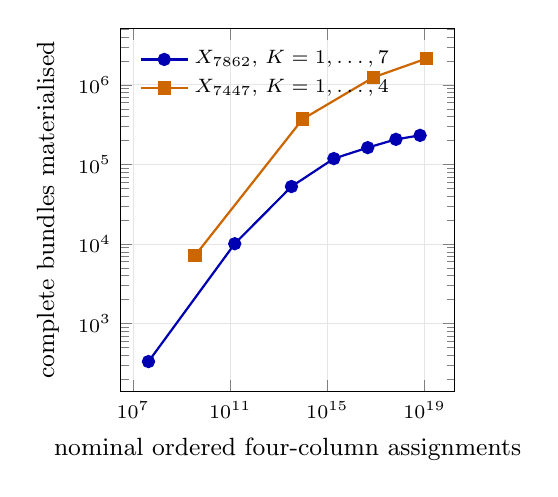
\begin{tikzpicture}
\begin{loglogaxis}[
  width=0.48\textwidth, height=6.2cm,
  xlabel={nominal ordered four-column assignments},
  ylabel={complete bundles materialised},
  legend pos=north west, legend style={font=\scriptsize, draw=none, fill=none},
  tick label style={font=\scriptsize}, label style={font=\small},
  grid=major, grid style={gray!20}]
\addplot[mark=*, thick, blue!70!black] coordinates {
  (4.30e7,334) (1.53e11,10097) (3.32e13,52800) (1.85e15,118577)
  (4.59e16,162761) (6.65e17,206847) (6.57e18,231946)};
\addlegendentry{$\Xa$, $K=1,\dots,7$}
\addplot[mark=square*, thick, orange!80!black] coordinates {
  (3.49e9,7122) (9.54e13,371214) (7.98e16,1245469) (1.22e19,2142164)};
\addlegendentry{$\Xb$, $K=1,\dots,4$}
\end{loglogaxis}
\end{tikzpicture}\hfill
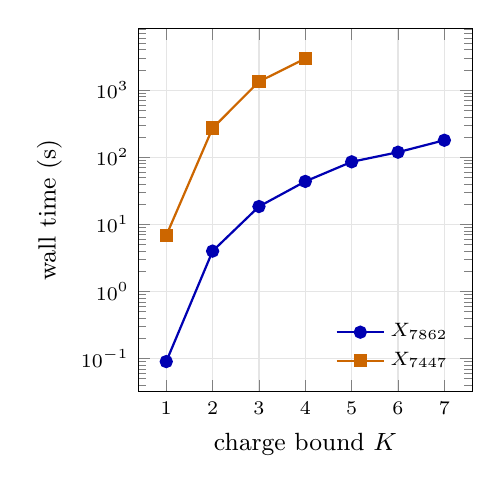
\begin{tikzpicture}
\begin{semilogyaxis}[
  width=0.48\textwidth, height=6.2cm,
  xlabel={charge bound $K$}, ylabel={wall time (s)},
  legend pos=south east, legend style={font=\scriptsize, draw=none, fill=none},
  tick label style={font=\scriptsize}, label style={font=\small},
  grid=major, grid style={gray!20}, xtick={1,2,3,4,5,6,7}]
\addplot[mark=*, thick, blue!70!black] coordinates {
  (1,0.09) (2,3.99) (3,18.42) (4,43.62) (5,85.44) (6,118.88) (7,179.15)};
\addlegendentry{$\Xa$}
\addplot[mark=square*, thick, orange!80!black] coordinates {
  (1,6.8) (2,271.6) (3,1338.8) (4,2960.2)};
\addlegendentry{$\Xb$}
\end{semilogyaxis}
\end{tikzpicture}
\caption{Left: the number of complete bundles the search actually builds against
the nominal size of the domain. Across eleven orders of magnitude in the domain
the materialised set grows by less than three, because the monotone rules prune
entire subtrees. Right: wall time on a single core ($\Gam=\Z_2$, complete slope
rule, bitset-indexed engine; the $\Xa$, $K=4$ point drops to 28.8\,s with the dual
slope decision).}
\label{fig:scaling}
\end{figure}

\Cref{fig:scaling} summarises the scaling. Three observations. First, the
materialised search space is essentially decoupled from the nominal one: on
$\Xa$ the nominal domain grows by a factor $1.5\times10^{11}$ from $K=1$ to $K=7$
while the bundles built grow by $7\times10^{2}$. Second, memory is not the
binding resource at this scale: peak resident memory is 189\,MiB at $\Xa$, $K=7$
and 706\,MiB at $\Xb$, $K=4$. Third, the cost of a node falls with depth because
of the dual slope decision (\cref{prop:dual}), so the dominant cost moves from
the slope test to enumeration as the search deepens.

Every escalation was preceded by a pilot and a written estimate: a $K=4$ pilot
on 8 roots predicted 110--450\,s against an actual 204.8\,s (before indexing),
and the $\Xb$ orbit counts at $K=2,3,4$ were predicted exactly from the
published catalog before the runs. For the downstairs stage, computing the
$\Gam$-representation on a 120-dimensional ambient cohomology group takes under
a second with the exact rational rank path.

The whole test suite---unit, differential (brute force against the split search
under all three slope-rule settings), certificate-replay and regression
tests---runs in about 30 seconds.

\section{Limitations and open problems}
\label{sec:limitations}

\paragraph{What is proved, and in what domain.} All \st{UNSAT\_BOUNDED} results
are statements about a declared finite domain, under the declared Kähler chamber
$T_+$ and the declared target. The slice results remove the charge bound only on
slices satisfying \eqref{eq:star}. The only statement with no domain qualifier
is the divisibility obstruction. Empirical saturation is not a theorem.

\paragraph{Generic members.} All cohomology is that of a Zariski-generic member
of the relevant family---the full family for upstairs statements, the
$\Gam$-invariant family for downstairs ones. Cohomology can jump on special
members, which can add vector-like pairs or singlets. The leading-order Yukawa
matrices are an exception: every coupling evaluated uses Koszul identifications
valid for every smooth member.

\paragraph{The Yukawa engine.} Triple products are computed for hypersurfaces in
products of $\PP^1$ and for bundles whose $H^1$ sits at a single Koszul level.
Couplings with Koszul level sum two or more, which need a lift through the
defining polynomial, and classes spread over both Koszul levels are returned as
\st{UNKNOWN}. Neither occurs among the Yukawa couplings of any model studied;
both occur for some one-singlet couplings $SLH_u$ of published models, which
are therefore reported as undecided. Couplings with singlet insertions are higher products, not triple
products, and are decided only by the selection rule. The normalisation of the
trace map and the matter Kähler metrics (for which a localisation approach
exists~\cite{BBCLP2018}) are not computed, so no physical Yukawa coupling or
fermion mass is claimed.

\paragraph{Scope of the group theory.} Only abelian $\Gam$ acting without
permuting projective factors is handled; non-abelian groups are refused. The
free action and invariant family are input from the published symmetry data.

\paragraph{Published-data discrepancies left open.} 954 of 2,007 published down-type Yukawa
tables are internally inconsistent as charge tables (\cref{sec:yukawa}); we
report this without reconciling it. (A second apparent discrepancy, in 694
character tables, turned out to be an error in our own comparison convention and
is resolved in \cref{sec:equivariant}.)

\paragraph{Not addressed.} Supersymmetry breaking, moduli stabilisation, the
full $F$- and $D$-flatness of singlet vacua away from vanishing FI terms, and
anything non-perturbative. Rules R2 and R3 restrict the domain to that of
\cite{ACGLP2013}; searches for models with anti-families or positive pair indices
would need them relaxed, which the replays show is supported but costly.

\paragraph{Open problems.}
\begin{enumerate}[leftmargin=*]
\item \emph{Finiteness on the tetraquadric.} Prove a charge bound on the slices
  where $F$ is indefinite, by bounding the semialgebraic set
  $\{F\le0,\ \ind\in[-3|\Gam|,0]\}$ using the cubic growth of the index along
  $F\le0$ rays; equivalently, settle \cref{conj:C1}.
\item \emph{Higher Koszul levels.} Extend the triple-product evaluation to
  level sum two, and to complete intersections of higher codimension, following
  the lifting construction of~\cite{BBCL2016,BBL2017}.
\item \emph{Singlet vacua.} Decide which singlet vacuum values are $F$- and
  $D$-flat away from the Abelian locus, and hence which of the
  \st{FULL\_RANK\_ON\_LOCUS} verdicts can be realised.
\item \emph{Rank below $h-1$.} Decide exactly the 18 extra survivors whose charge
  matrix has rank below $h-1$, where the slope-zero locus is positive-dimensional
  and \cref{prop:decision} does not apply; and push the survey of
  \cref{sec:survey} to larger $K$, where more models missing from the catalog may
  appear.
\end{enumerate}

\section{Conclusions}
\label{sec:conclusions}

We have built a search for heterotic line-bundle models in which every pruning
step is a theorem with stated assumptions, and used it to push the analysis from
the upstairs GUT stage through the equivariant descent to the holomorphic
superpotential.

On the side of \emph{search}, the central observation is that the slope
obstruction, used in earlier scans as a finite coefficient test, has an exact
and complete form---a fixed polyhedral cone meeting the span of the charge
vectors---that is monotone, prunes every branch, and is decided by a dual test
whose cost falls with depth. It removes a spurious candidate the finite test
keeps, and with it the search reproduces the published catalogs of both
benchmark geometries exactly. The slice decomposition that follows from the same
geometry turns 425 slices of the tetraquadric into theorems valid for
arbitrarily large charges, and isolates precisely the slices where only the
cubic growth of the index can bound the charges. Run over all 68 favourable
CICYs, the search never misses a published model, and an exact decision of
stability---validated by never rejecting one---shows that the published catalog
itself is incomplete: it lacks at least one poly-stable GUT model whose only
stability witness lies at a Kähler class with moduli ratio about 1:231.

On the side of \emph{physics}, computing the $\Gam$-representation on cohomology
from the group action lets the pipeline discover rather than verify: from our
own exhaustive survivor set it recovers all ten published standard-model orbits
on the tetraquadric quotient and finds eleven more. Their absence from the
published database is explained, in every case, by restrictions the published
scan states for itself. The superpotential machinery reproduces every operator
table of that database, exposes an internal inconsistency in almost half of its
down-type Yukawa tables, and---by evaluating leading-order couplings as genuine
triple products---detects vanishings that charge conservation cannot.

The answer to the phenomenological question is sobering and, we think, useful:
no model on this quotient, published or new, combines a leading-order top Yukawa
with rank-three Yukawa matrices and the absence of dangerous operators. The new
models fail in the same ways and at a comparable rate as the published ones. Two
of them (A04, A06) remain open, and deciding them requires exactly the
ingredients---higher-order couplings, singlet vacua, Kähler metrics---whose
absence we have documented rather than papered over.

The methods are not specific to the two benchmarks, as the run over all 68
favourable CICYs shows: the complete slope test needs only the triple
intersection numbers, the exact stability decision only the slopes, and the flow
formulation of the selection rules is geometry-independent. The natural next
steps are that survey at larger charges---where more models missing from the
catalog may appear---the exact treatment of rank-deficient charge matrices, the
extension of the triple-product evaluation to higher Koszul levels, and the
finiteness question of \cref{conj:C1}.


\appendix
\section{Reproducibility}
\label{app:reproducibility}

Everything in this paper is produced by the accompanying repository, which needs
only Python and uses exact integer and rational arithmetic throughout; no
computer-algebra system or external cohomology package is required. Raw inputs
(the published catalogs \texttt{GUTall.m} and \texttt{sms202.m} and the symmetry
data) are stored with SHA-256 checksums. Every search run writes a checkpointed
JSON artifact embedding the hash of the source and inputs, and refuses to resume
under changed code. The test suite (255 tests: unit, differential, certificate
replay and regression tests pinning every number reported here) runs in about
30 seconds.

\begin{center}\small
\begin{tabular}{@{}p{0.47\textwidth}p{0.47\textwidth}@{}}
\toprule
result & command (from the repository root) \\
\midrule
bounded search, e.g.\ $\Xa$, $K=3$ &
\texttt{python -m string\_sm\_sat.cli search -{}-geometry 7862 -{}-K 3 -{}-gamma 2 -{}-slope-rule span} \\
independent replay (\cref{tab:replay}) & \texttt{scripts/independent\_replay.py} \\
catalog comparison (\cref{tab:catalog}) & \texttt{scripts/compare\_catalog.py} \\
charge-unbounded slices (\cref{sec:slices}) & \texttt{scripts/slice\_certificate.py} \\
equivariant cohomology (\cref{sec:equivariant}) & \texttt{scripts/compute\_equivariant\_cohomology.py} \\
downstairs search (\cref{sec:downstairs}) & \texttt{scripts/search\_standard\_models.py} \\
candidate audit and absence resolution & \texttt{scripts/audit\_candidates.py}, \texttt{scripts/absence\_resolution.py} \\
Yukawa and operator tables (\cref{tab:operators}) & \texttt{scripts/yukawa\_selection\_benchmark.py}, \texttt{operator\_benchmark.py}, \texttt{kahler\_benchmark.py} \\
internal consistency of published tables & \texttt{scripts/published\_table\_consistency.py} \\
leading-order ranks & \texttt{scripts/leading\_order\_yukawa.py} \\
singlet-spectrum validation & \texttt{scripts/validate\_singlet\_spectrum.py} \\
candidate Yukawa sector and ranking (\cref{tab:ranking}) & \texttt{scripts/candidate\_yukawa.py}, \texttt{scripts/rank\_candidates.py} \\
68-geometry survey (\cref{tab:survey}) & \texttt{scripts/phase8\_suite.py}, \texttt{phase8\_extras.py} \\
the new GUT model & \texttt{scripts/new\_gut\_model\_certificate.py} \\
\bottomrule
\end{tabular}
\end{center}

The append-only research notebook \texttt{RESULTS.md} records every run with its
statistics, including corrections to earlier entries; the mathematical notes in
\texttt{docs/} give the full proofs summarised here.

\section{Conventions and source discrepancies}
\label{app:conventions}

\paragraph{Topology.} Indices mean $\chi=\sum_q(-1)^qh^q$; $J_i$ are the ordered
restricted hyperplane classes; $d_{ijl}$ integrates $J_iJ_jJ_l$ and $c_{2,i}$
pairs $c_2(TX)$ with $J_i$. For $c_1(V)=0$, $c_2(V)=-\tfrac12\sum_ak_a^2$ (Whitney);
the positive quadratic expression called $c_2(V)$ in \cite[Sec.~5]{ACGLP2013}
is $\mathrm{ch}_2(V)$, and we follow the sign of \cite[(2.3)]{BCL2013}, confirmed by
the published example.

\paragraph{Published data.} Published charge matrices are stored with rows
indexed by ambient factors; we transpose to columns. The character tables
\texttt{GCoh} are indexed by characters in lexicographic label order, with
$\Gam$ inferred database-wide, and are raw characters of the lift, before the
equivariant shift. The equivariant structure enters as a character
shift, $\chi_a$ for $L_a$ and $\chi_a+\chi_b$ for $L_aL_b$ (fixed by the data:
1,948/1,948 spectra with the shift, 1,503 without).
\texttt{EDownSpec[[1]]} is
$[H_u\text{ pair},\ \text{three }\ten\text{ bundles},\ H_d\text{ pair},\ \text{three
}\bfive\text{ pairs},\ \text{singlet codes}]$ with pair index the position among
the ten lexicographic pairs and singlet code $2\cdot(\text{pair index})+\text{direction}$;
\texttt{EDownSpec[[2]]} lists the Higgs slots. In the text of \cite{AGLP2012}
$\bar H$ denotes the up-type Higgs, while the database field
\texttt{Subscript["H",a,b]} is the $\five$ (up-type); both readings are needed to
map the Kähler operators correctly.

\paragraph{Discrepancies in the sources, recorded and not silently corrected.}
\begin{itemize}[leftmargin=*]
\item \cite{ACHLN2023} prints a positive chiral Euler characteristic in one
  condition while its objective uses the negative target; we follow HRR and the
  published cohomology.
\item \cite[Sec.~7]{ACGLP2013} describes the ranks of $V$ and $TX$ as equal
  (they are five and three); we reproduce $c_2$ equality only.
\item The GUT catalog lists symmetry orders $\{2,4,5,10,20\}$ for CICY 7447
  while the symmetry pages list $\{2,4,10\}$; no result depends on it, and order
  5 is excluded independently by \cref{prop:divisibility}.
\item 954 of 2,007 published down-type Yukawa tables are not functions of the
  charges (\cref{sec:yukawa}), and the published \texttt{Dim5Proton} tables list
  an inconsistent subset of index permutations.
\item The singlet multiplicities of 2,450 entries across 1,197 published records
  are unevaluated rank expressions; where we evaluate one (CICY 7862, model 2) we
  find zero at a generic invariant member.
\end{itemize}


\section*{Acknowledgements}
[To be completed.] The computations use only exact integer and rational
arithmetic and open-source Python; no computer-algebra system or external
cohomology package is required.

\bibliographystyle{unsrt}
\bibliography{references}

\end{document}
